\pagebreak
\section{Wyniki eksperytmentu}

\subsection{Zbiór "Diabetes"}
  \begin{figure}[H]
    \center
    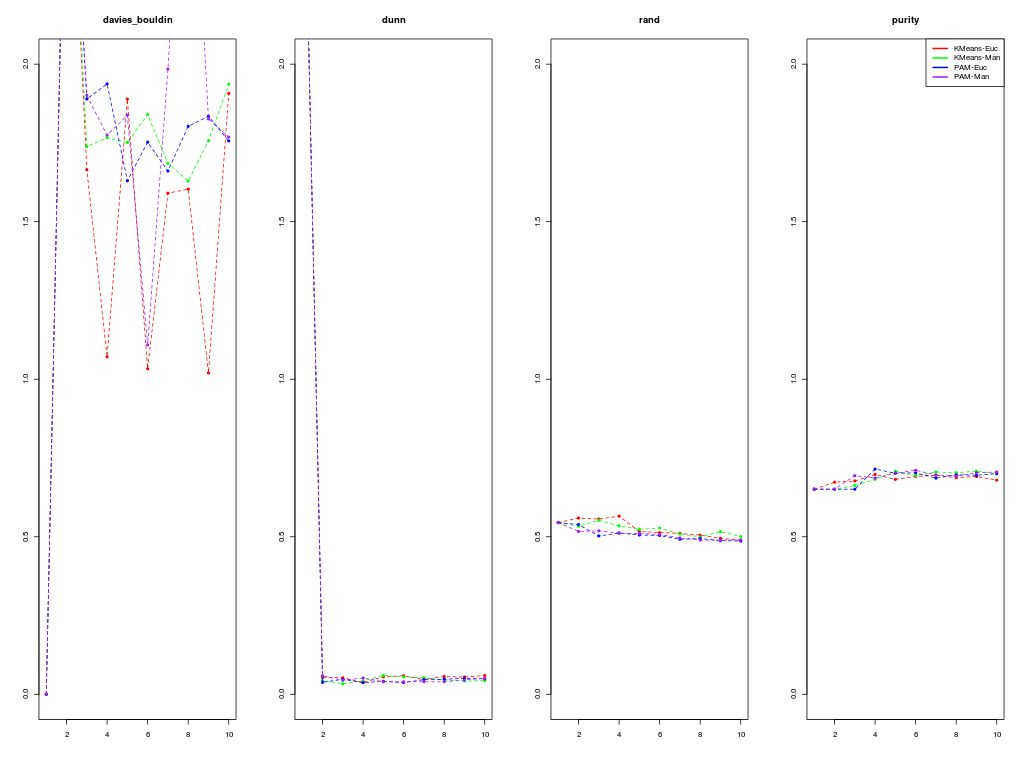
\includegraphics[width=\textwidth]{resources/plots/diabetes_metrics.png}
    \caption{Wykresy wartości metryk dla zbioru "Diabetes".}
  \end{figure}

  % latex table generated in R 3.4.4 by xtable 1.8-2 package
% Sun May  6 16:29:09 2018
\begin{table}[ht]
\centering
\begin{tabular}{llrlrr}
  \hline
alg & nb\_clus & davies\_bouldin & dunn & rand & purity \\ 
  \hline
KMeans-Euc & 1 & 0.00 & INF & 0.55 & 0.65 \\ 
  KMeans-Euc & 2 & 2.01 & 0.053 & 0.56 & 0.67 \\ 
  KMeans-Euc & 3 & 1.67 & 0.052 & 0.56 & 0.68 \\ 
  KMeans-Euc & 4 & 1.07 & 0.038 & 0.57 & 0.70 \\ 
  KMeans-Euc & 5 & 1.89 & 0.056 & 0.52 & 0.68 \\ 
  KMeans-Euc & 6 & 1.03 & 0.059 & 0.51 & 0.69 \\ 
  KMeans-Euc & 7 & 1.59 & 0.048 & 0.51 & 0.69 \\ 
  KMeans-Euc & 8 & 1.60 & 0.056 & 0.51 & 0.69 \\ 
  KMeans-Euc & 9 & 1.02 & 0.055 & 0.49 & 0.69 \\ 
  KMeans-Euc & 10 & 1.91 & 0.06 & 0.49 & 0.68 \\ 
  KMeans-Man & 1 & 0.00 & INF & 0.55 & 0.65 \\ 
  KMeans-Man & 2 & 2.16 & 0.043 & 0.53 & 0.65 \\ 
  KMeans-Man & 3 & 1.74 & 0.034 & 0.55 & 0.66 \\ 
  KMeans-Man & 4 & 1.77 & 0.043 & 0.54 & 0.68 \\ 
  KMeans-Man & 5 & 1.75 & 0.06 & 0.52 & 0.71 \\ 
  KMeans-Man & 6 & 1.84 & 0.056 & 0.53 & 0.69 \\ 
  KMeans-Man & 7 & 1.69 & 0.052 & 0.51 & 0.71 \\ 
  KMeans-Man & 8 & 1.63 & 0.046 & 0.50 & 0.70 \\ 
  KMeans-Man & 9 & 1.76 & 0.042 & 0.52 & 0.71 \\ 
  KMeans-Man & 10 & 1.94 & 0.043 & 0.50 & 0.70 \\ 
  PAM-Euc & 1 & 0.00 & INF & 0.55 & 0.65 \\ 
  PAM-Euc & 2 & 2.19 & 0.038 & 0.54 & 0.65 \\ 
  PAM-Euc & 3 & 1.89 & 0.048 & 0.50 & 0.65 \\ 
  PAM-Euc & 4 & 1.94 & 0.037 & 0.51 & 0.71 \\ 
  PAM-Euc & 5 & 1.63 & 0.041 & 0.51 & 0.70 \\ 
  PAM-Euc & 6 & 1.75 & 0.037 & 0.50 & 0.70 \\ 
  PAM-Euc & 7 & 1.66 & 0.047 & 0.49 & 0.69 \\ 
  PAM-Euc & 8 & 1.80 & 0.048 & 0.49 & 0.70 \\ 
  PAM-Euc & 9 & 1.83 & 0.051 & 0.49 & 0.69 \\ 
  PAM-Euc & 10 & 1.76 & 0.049 & 0.49 & 0.70 \\ 
  PAM-Man & 1 & 0.00 & INF & 0.55 & 0.65 \\ 
  PAM-Man & 2 & 2.35 & 0.058 & 0.52 & 0.65 \\ 
  PAM-Man & 3 & 1.90 & 0.045 & 0.52 & 0.69 \\ 
  PAM-Man & 4 & 1.77 & 0.052 & 0.51 & 0.69 \\ 
  PAM-Man & 5 & 1.84 & 0.04 & 0.51 & 0.70 \\ 
  PAM-Man & 6 & 1.11 & 0.04 & 0.51 & 0.71 \\ 
  PAM-Man & 7 & 1.98 & 0.04 & 0.50 & 0.70 \\ 
  PAM-Man & 8 & 2.02 & 0.04 & 0.49 & 0.69 \\ 
  PAM-Man & 9 & 1.83 & 0.046 & 0.49 & 0.70 \\ 
  PAM-Man & 10 & 1.77 & 0.051 & 0.49 & 0.71 \\ 
   \hline
\end{tabular}
\end{table}


  \subsubsection{Algorytm K-Means (Euclidean)} 
    \begin{figure}[H]
      \center
      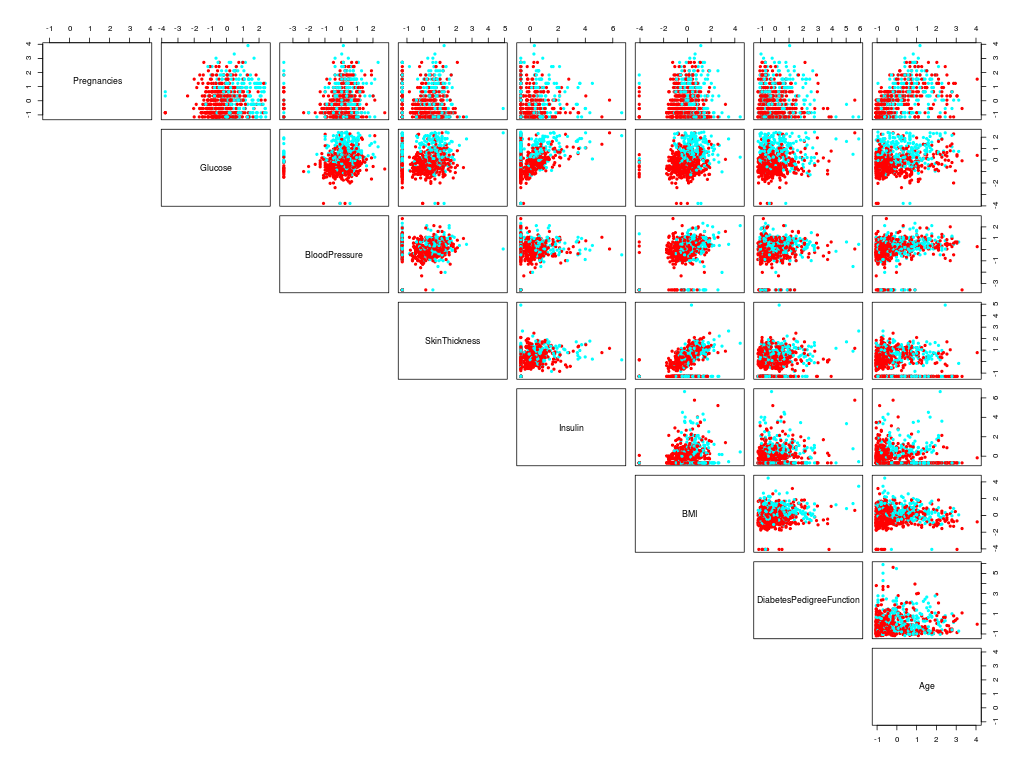
\includegraphics[width=0.8\textwidth]{resources/plots/diabetes_KMeans-Euc_scatter.png}
      \caption{Wynik klasteryzacji dla algorytmu KMeans (Euclidean) dla zbioru "Diabetes".}
    \end{figure}
    \begin{figure}[H]
      \center
      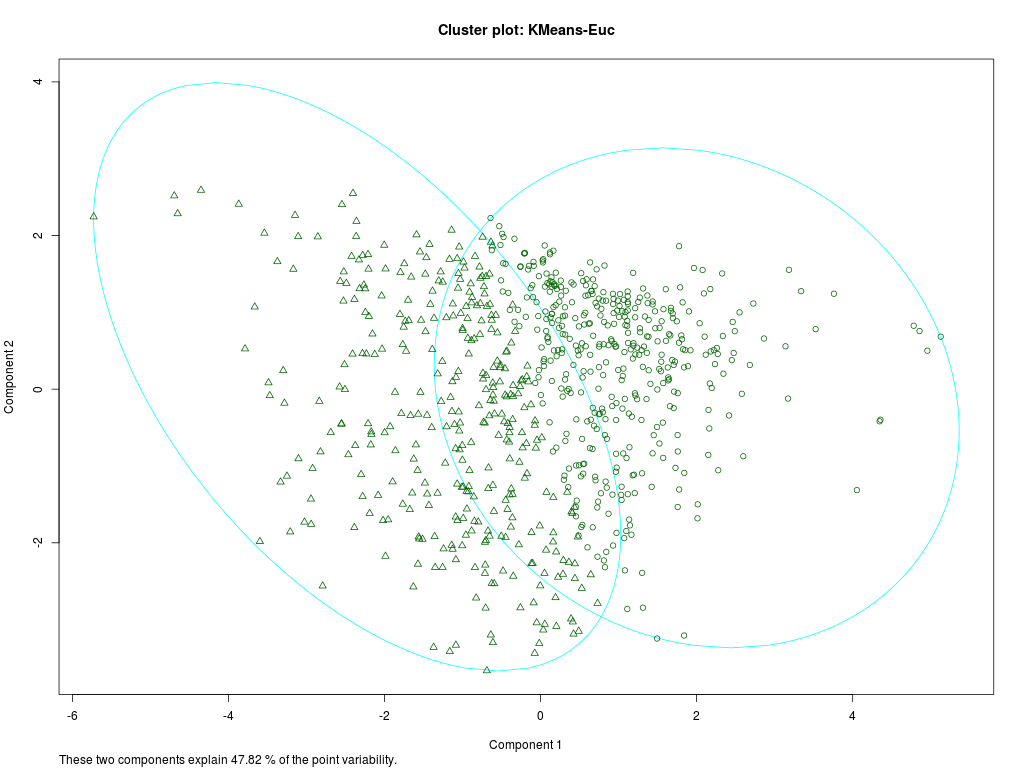
\includegraphics[width=0.8\textwidth]{resources/plots/diabetes_KMeans-Euc_cluster.png}
      \caption{Klastry dla algorytmu KMeans (Euclidean) dla zbioru "Diabetes".}
    \end{figure}

  \subsubsection{Algorytm K-Means (Manhattan)} 
    \begin{figure}[H]
      \center
      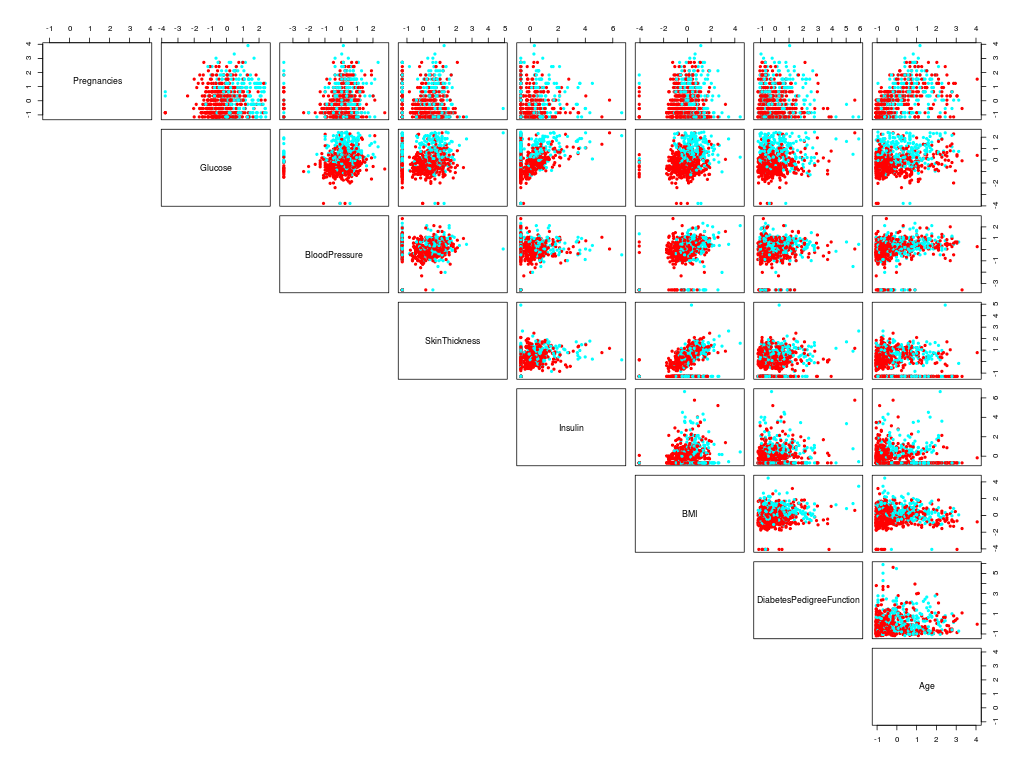
\includegraphics[width=0.8\textwidth]{resources/plots/diabetes_KMeans-Man_scatter.png}
      \caption{Wynik klasteryzacji dla algorytmu KMeans (Manhattan) dla zbioru "Diabetes".}
    \end{figure}
    \begin{figure}[H]
      \center
      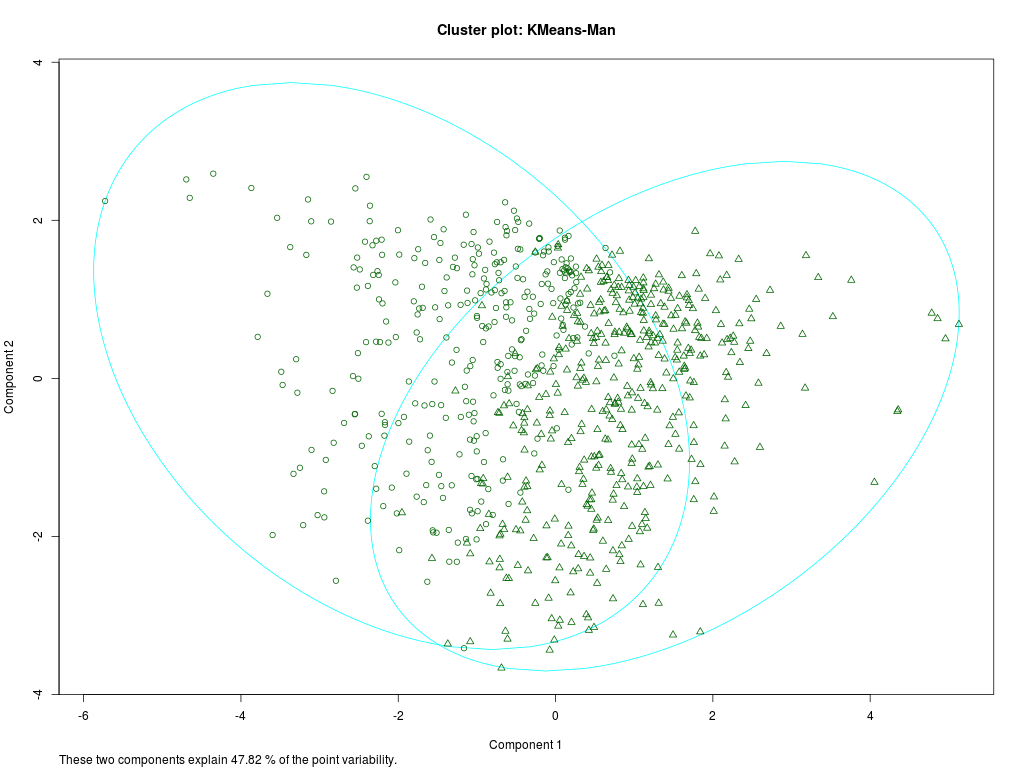
\includegraphics[width=0.8\textwidth]{resources/plots/diabetes_KMeans-Man_cluster.png}
      \caption{Klastry dla algorytmu KMeans (Manhattan) dla zbioru "Diabetes".}
    \end{figure}

  \subsubsection{Algorytm PAM (Euclidean)} 
    \begin{figure}[H]
      \center
      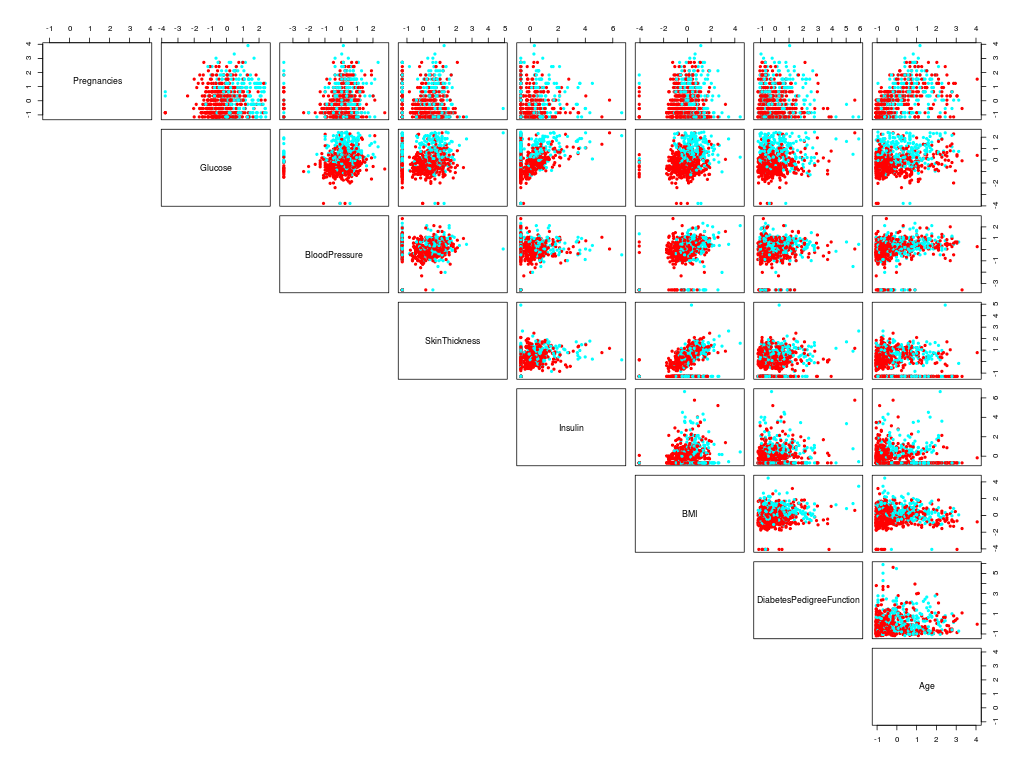
\includegraphics[width=0.8\textwidth]{resources/plots/diabetes_PAM-Euc_scatter.png}
      \caption{Wynik klasteryzacji dla algorytmu PAM (Euclidean) dla zbioru "Diabetes".}
    \end{figure}
    \begin{figure}[H]
      \center
      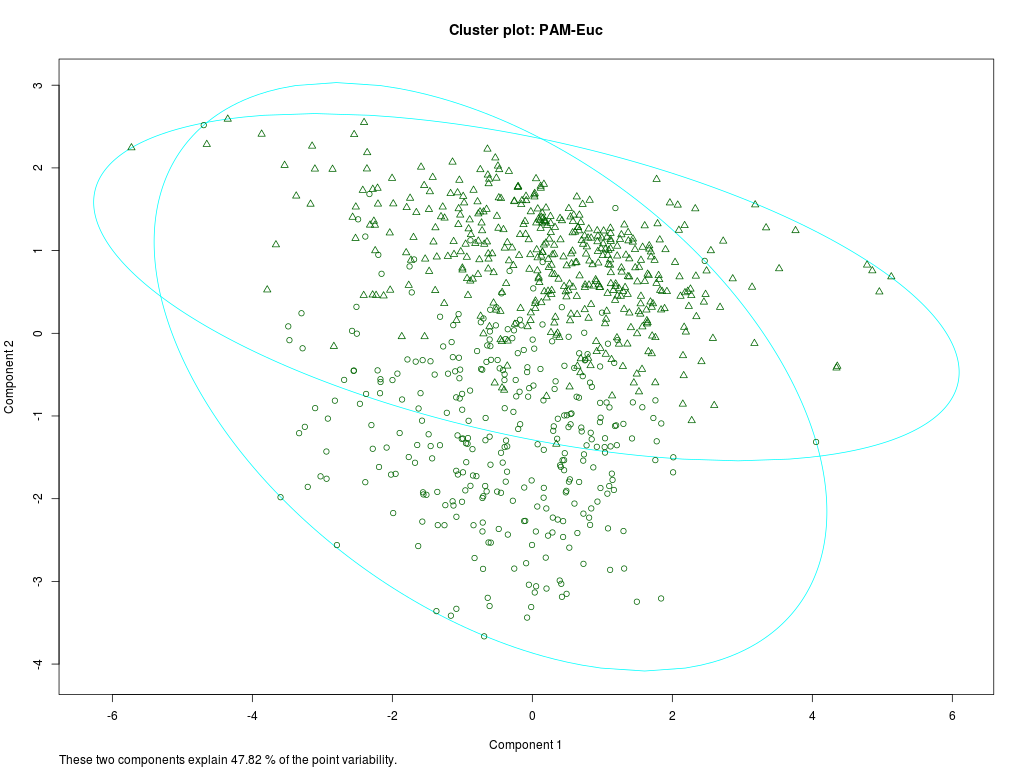
\includegraphics[width=0.8\textwidth]{resources/plots/diabetes_PAM-Euc_cluster.png}
      \caption{Klastry dla algorytmu PAM (Euclidean) dla zbioru "Diabetes".}
    \end{figure}

  \subsubsection{Algorytm PAM (Manhattan)} 
    \begin{figure}[H]
      \center
      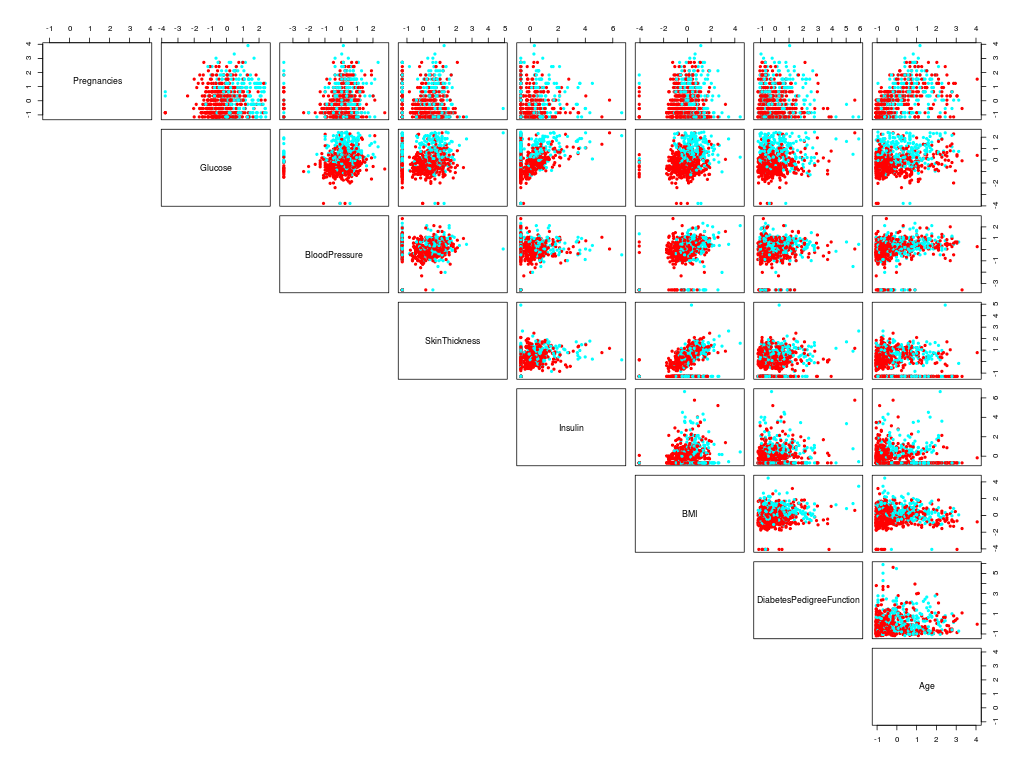
\includegraphics[width=0.8\textwidth]{resources/plots/diabetes_PAM-Man_scatter.png}
      \caption{Wynik klasteryzacji dla algorytmu PAM (Manhattan) dla zbioru "Diabetes".}
    \end{figure}
    \begin{figure}[H]
      \center
      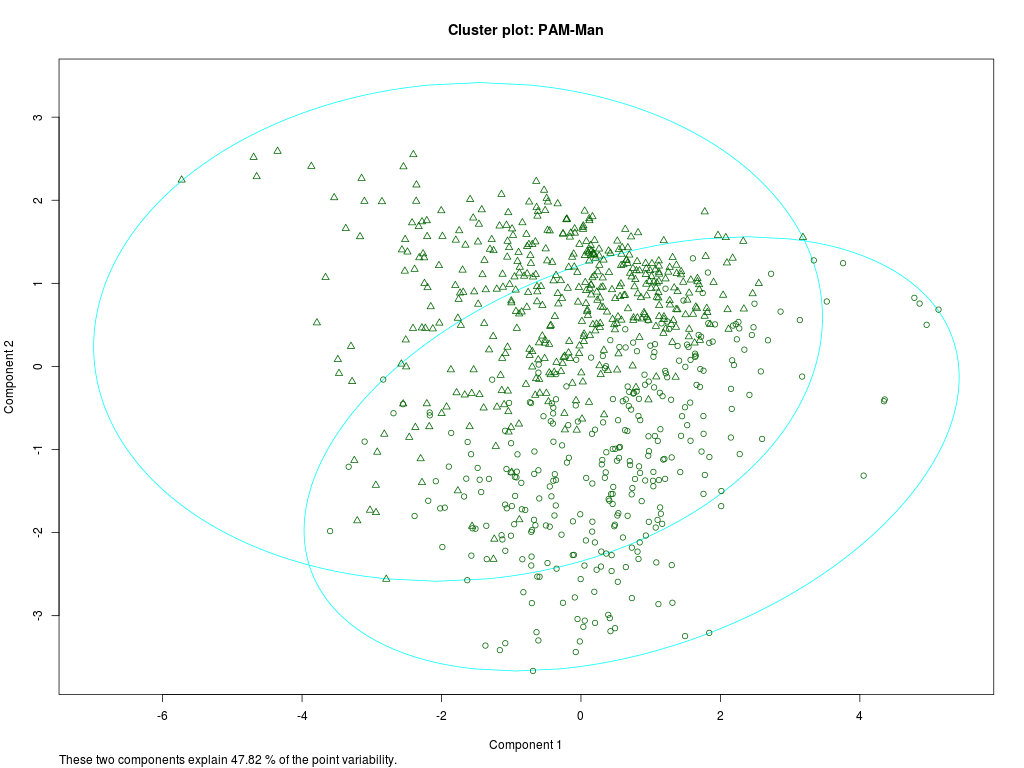
\includegraphics[width=0.8\textwidth]{resources/plots/diabetes_PAM-Man_cluster.png}
      \caption{Klastry dla algorytmu PAM (Manhattan) dla zbioru "Diabetes".}
    \end{figure}

\subsection{Zbiór "Glass"}
  \begin{figure}[H]
    \center
    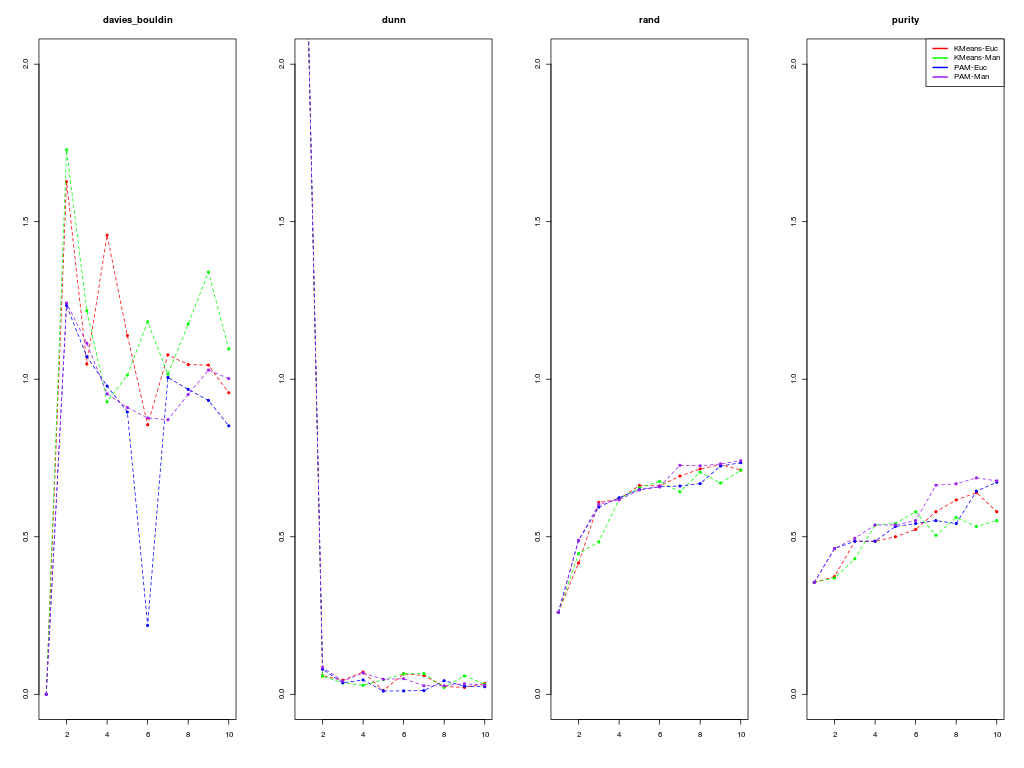
\includegraphics[width=\textwidth]{resources/plots/glass_metrics.png}
    \caption{Wykresy wartości metryk dla zbioru "Glass".}
  \end{figure}

  % latex table generated in R 3.4.4 by xtable 1.8-2 package
% Sun May  6 16:30:11 2018
\begin{table}[H]
\centering
\begin{tabular}{cc|cccc}
  \hline
Algorytm & Liczba klastrów & davies\_bouldin & dunn & rand & purity \\ 
  \hline
  \multirow{10}{*}{KMeans-Euc} & 1 & 0.00 & INF & 0.26 & 0.35 \\ 
   & 2 & 1.63 & 0.058 & 0.42 & 0.37 \\ 
   & 3 & 1.05 & 0.045 & 0.61 & 0.49 \\ 
   & 4 & 1.46 & 0.071 & 0.62 & 0.49 \\ 
   & 5 & 1.14 & 0.012 & 0.66 & 0.50 \\ 
   & 6 & 0.85 & 0.065 & 0.66 & 0.52 \\ 
   & 7 & 1.08 & 0.06 & 0.69 & 0.58 \\ 
   & 8 & 1.05 & 0.025 & 0.71 & 0.62 \\ 
   & 9 & 1.04 & 0.022 & 0.73 & 0.64 \\ 
   & 10 & 0.96 & 0.035 & 0.71 & 0.58 \\ \hline \hline 
  \multirow{10}{*}{KMeans-Man} & 1 & 0.00 & INF & 0.26 & 0.35 \\ 
  & 2 & 1.73 & 0.058 & 0.45 & 0.37 \\ 
  & 3 & 1.22 & 0.036 & 0.48 & 0.43 \\ 
  & 4 & 0.93 & 0.029 & 0.62 & 0.54 \\ 
  & 5 & 1.01 & 0.046 & 0.66 & 0.54 \\ 
  & 6 & 1.18 & 0.065 & 0.68 & 0.58 \\ 
  & 7 & 1.02 & 0.066 & 0.64 & 0.51 \\ 
  & 8 & 1.18 & 0.022 & 0.70 & 0.56 \\ 
  & 9 & 1.34 & 0.058 & 0.67 & 0.53 \\ 
  & 10 & 1.10 & 0.032 & 0.71 & 0.55 \\ \hline \hline
  \multirow{10}{*}{PAM-Euc} & 1 & 0.00 & INF & 0.26 & 0.35 \\ 
  & 2 & 1.23 & 0.08 & 0.49 & 0.46 \\ 
  & 3 & 1.07 & 0.037 & 0.59 & 0.49 \\ 
  & 4 & 0.98 & 0.046 & 0.62 & 0.49 \\ 
  & 5 & 0.90 & 0.01 & 0.65 & 0.53 \\ 
  & 6 & 0.22 & 0.011 & 0.66 & 0.54 \\ 
  & 7 & 1.01 & 0.012 & 0.66 & 0.55 \\ 
  & 8 & 0.97 & 0.043 & 0.67 & 0.54 \\ 
  & 9 & 0.93 & 0.026 & 0.72 & 0.65 \\ 
  & 10 & 0.85 & 0.024 & 0.73 & 0.67 \\ \hline \hline
  \multirow{10}{*}{PAM-Man} & 1 & 0.00 & INF & 0.26 & 0.35 \\ 
  & 2 & 1.24 & 0.086 & 0.49 & 0.46 \\ 
  & 3 & 1.11 & 0.042 & 0.60 & 0.49 \\ 
  & 4 & 0.95 & 0.067 & 0.62 & 0.54 \\ 
  & 5 & 0.91 & 0.048 & 0.65 & 0.54 \\ 
  & 6 & 0.88 & 0.05 & 0.66 & 0.55 \\ 
  & 7 & 0.87 & 0.027 & 0.73 & 0.66 \\ 
  & 8 & 0.95 & 0.027 & 0.72 & 0.67 \\ 
  & 9 & 1.03 & 0.034 & 0.73 & 0.69 \\ 
  & 10 & 1.00 & 0.029 & 0.74 & 0.68 \\ 
   \hline
\end{tabular}
  \caption{Wartości metryk dla zbioru "Glass".}
\end{table}


  \subsubsection{Algorytm K-Means (Euclidean)} 
    \begin{figure}[H]
      \center
      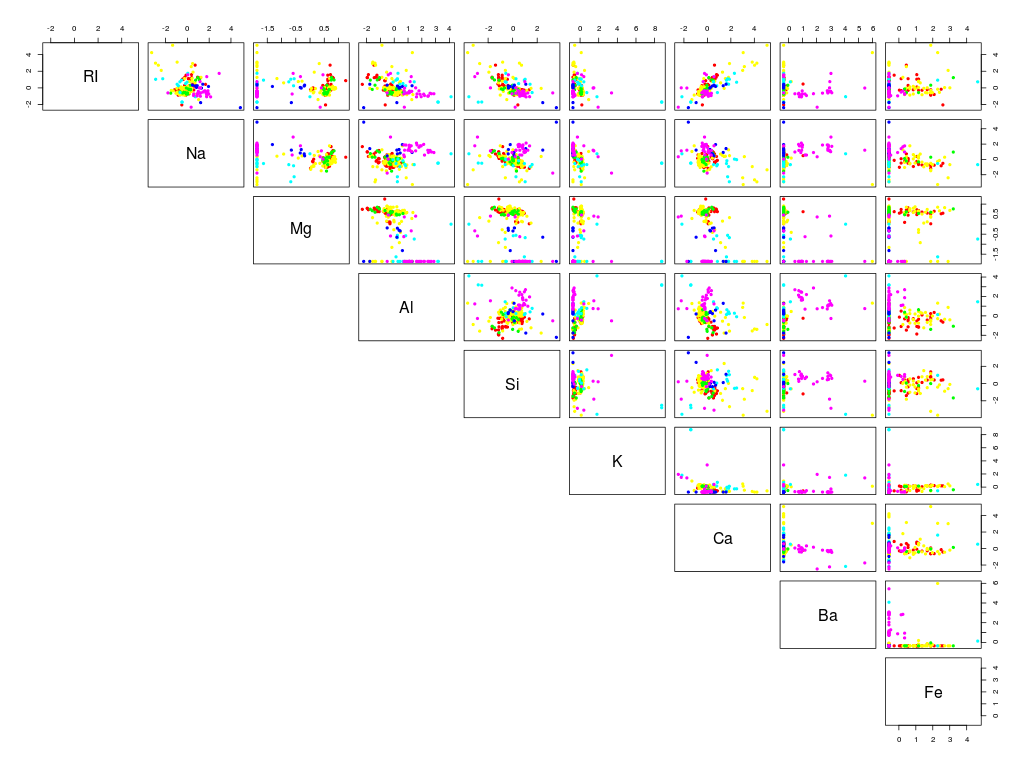
\includegraphics[width=0.8\textwidth]{resources/plots/glass_KMeans-Euc_scatter.png}
      \caption{Wynik klasteryzacji dla algorytmu KMeans (Euclidean) dla zbioru "Glass".}
    \end{figure}
    \begin{figure}[H]
      \center
      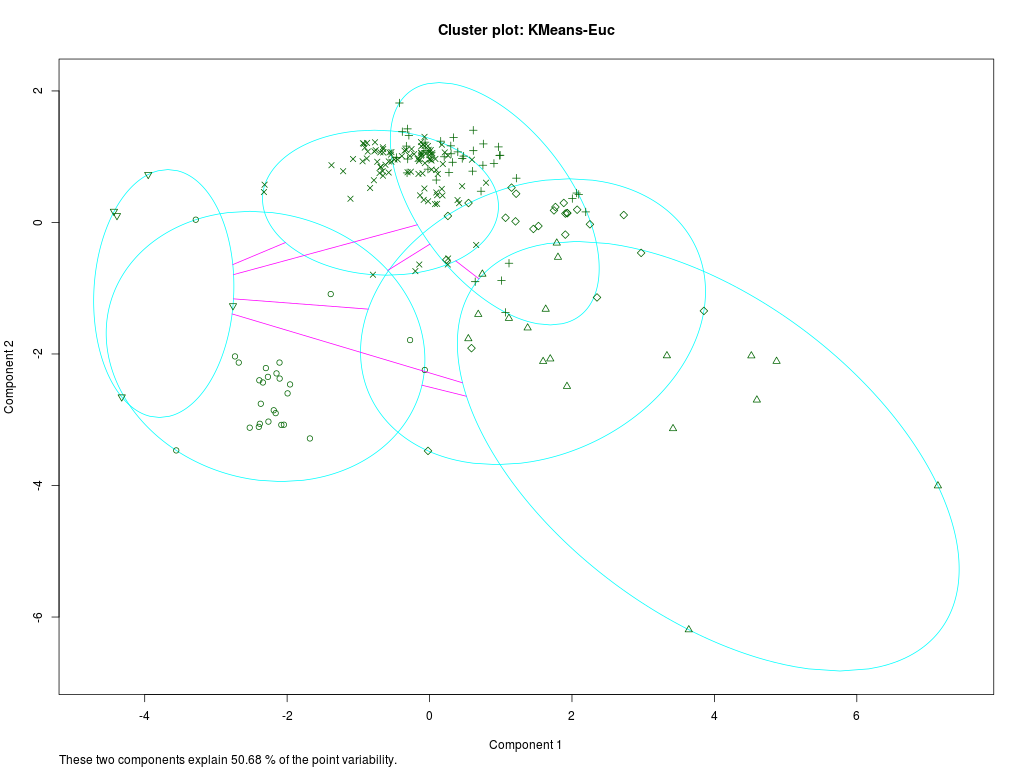
\includegraphics[width=0.8\textwidth]{resources/plots/glass_KMeans-Euc_cluster.png}
      \caption{Klastry dla algorytmu KMeans (Euclidean) dla zbioru "Glass".}
    \end{figure}

  \subsubsection{Algorytm K-Means (Manhattan)} 
    \begin{figure}[H]
      \center
      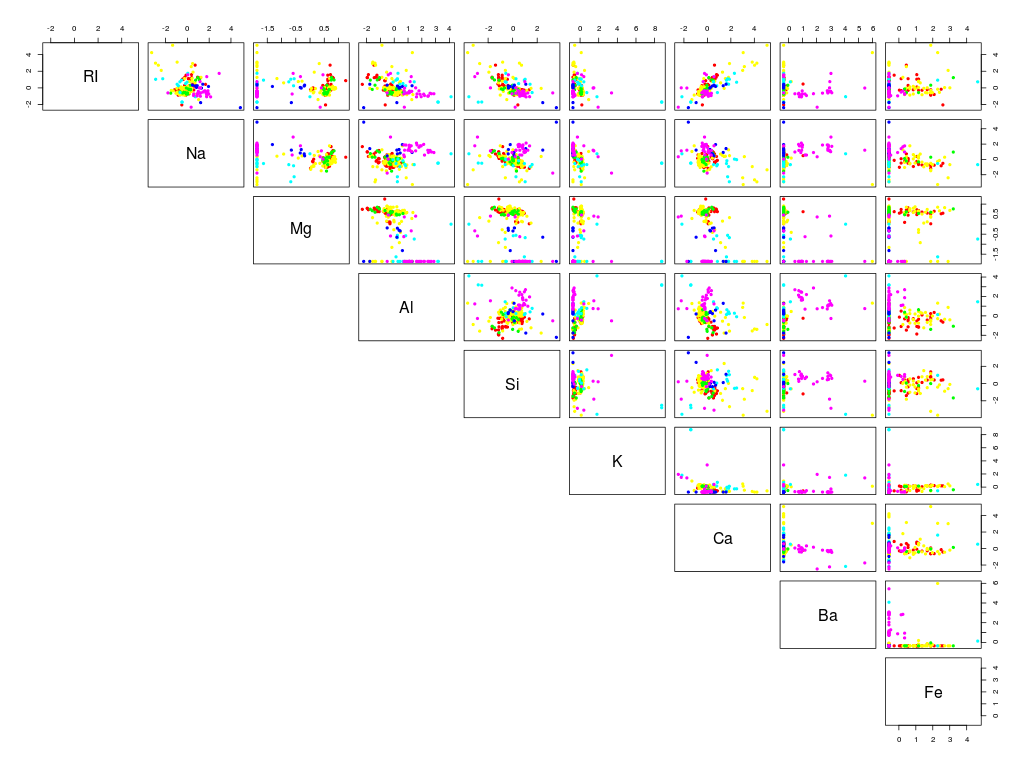
\includegraphics[width=0.8\textwidth]{resources/plots/glass_KMeans-Man_scatter.png}
      \caption{Wynik klasteryzacji dla algorytmu KMeans (Manhattan) dla zbioru "Glass".}
    \end{figure}
    \begin{figure}[H]
      \center
      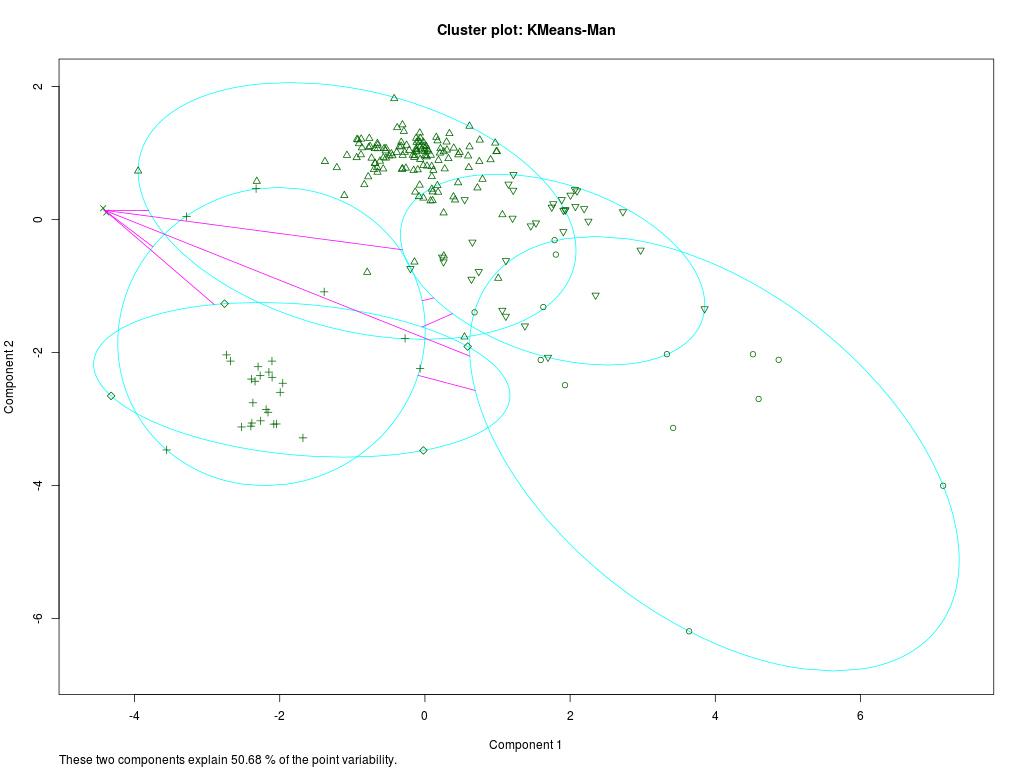
\includegraphics[width=0.8\textwidth]{resources/plots/glass_KMeans-Man_cluster.png}
      \caption{Klastry dla algorytmu KMeans (Manhattan) dla zbioru "Glass".}
    \end{figure}

  \subsubsection{Algorytm PAM (Euclidean)} 
    \begin{figure}[H]
      \center
      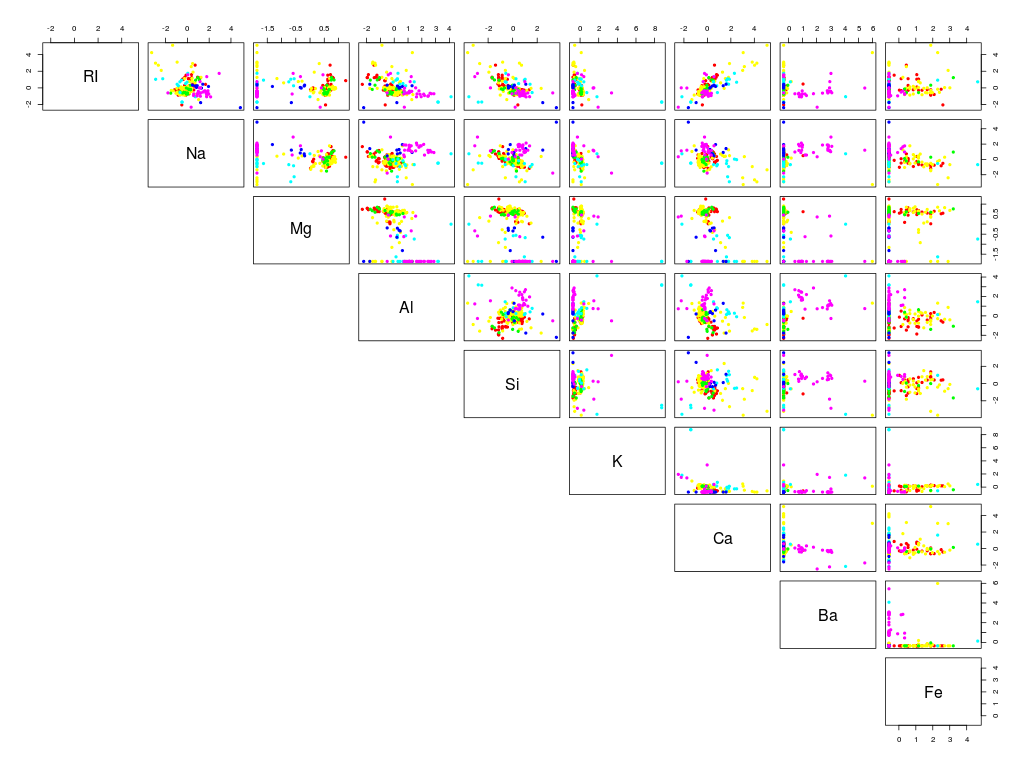
\includegraphics[width=0.8\textwidth]{resources/plots/glass_PAM-Euc_scatter.png}
      \caption{Wynik klasteryzacji dla algorytmu PAM (Euclidean) dla zbioru "Glass".}
    \end{figure}
    \begin{figure}[H]
      \center
      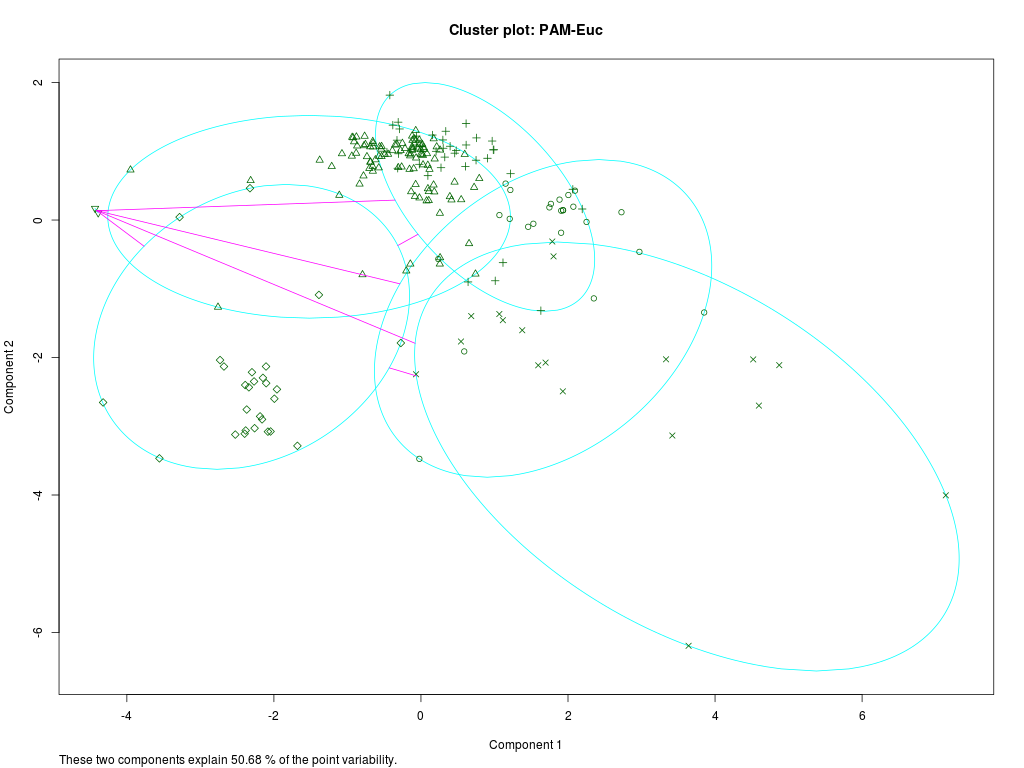
\includegraphics[width=0.8\textwidth]{resources/plots/glass_PAM-Euc_cluster.png}
      \caption{Klastry dla algorytmu PAM (Euclidean) dla zbioru "Glass".}
    \end{figure}

  \subsubsection{Algorytm PAM (Manhattan)} 
    \begin{figure}[H]
      \center
      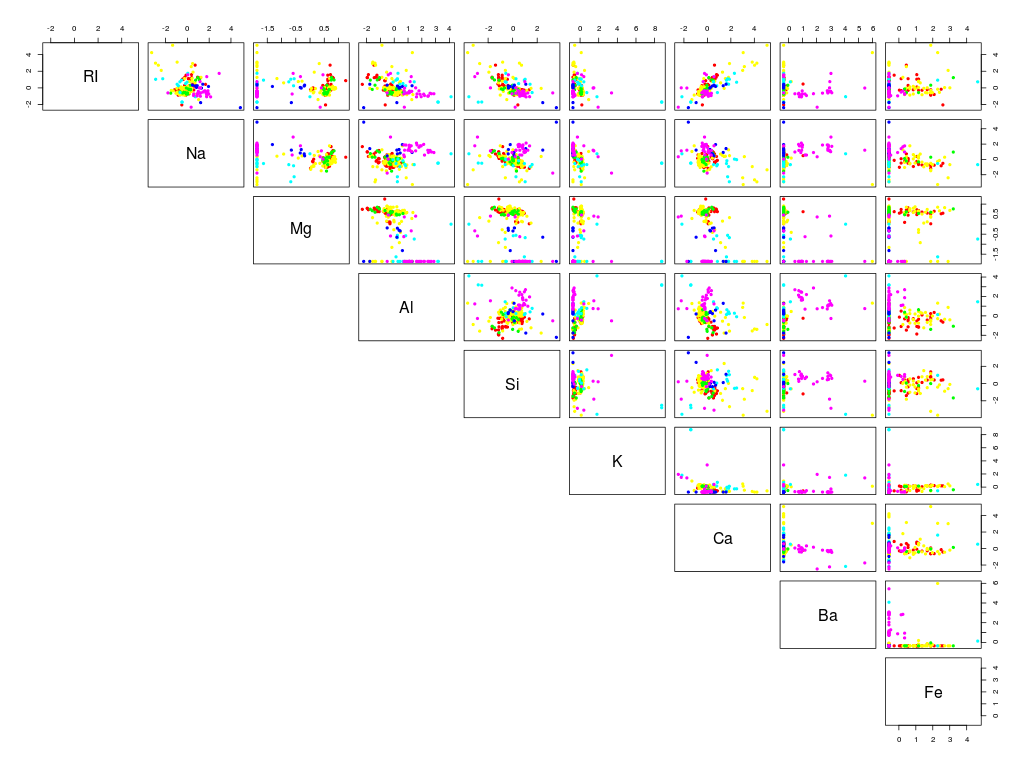
\includegraphics[width=0.8\textwidth]{resources/plots/glass_PAM-Man_scatter.png}
      \caption{Wynik klasteryzacji dla algorytmu PAM (Manhattan) dla zbioru "Glass".}
    \end{figure}
    \begin{figure}[H]
      \center
      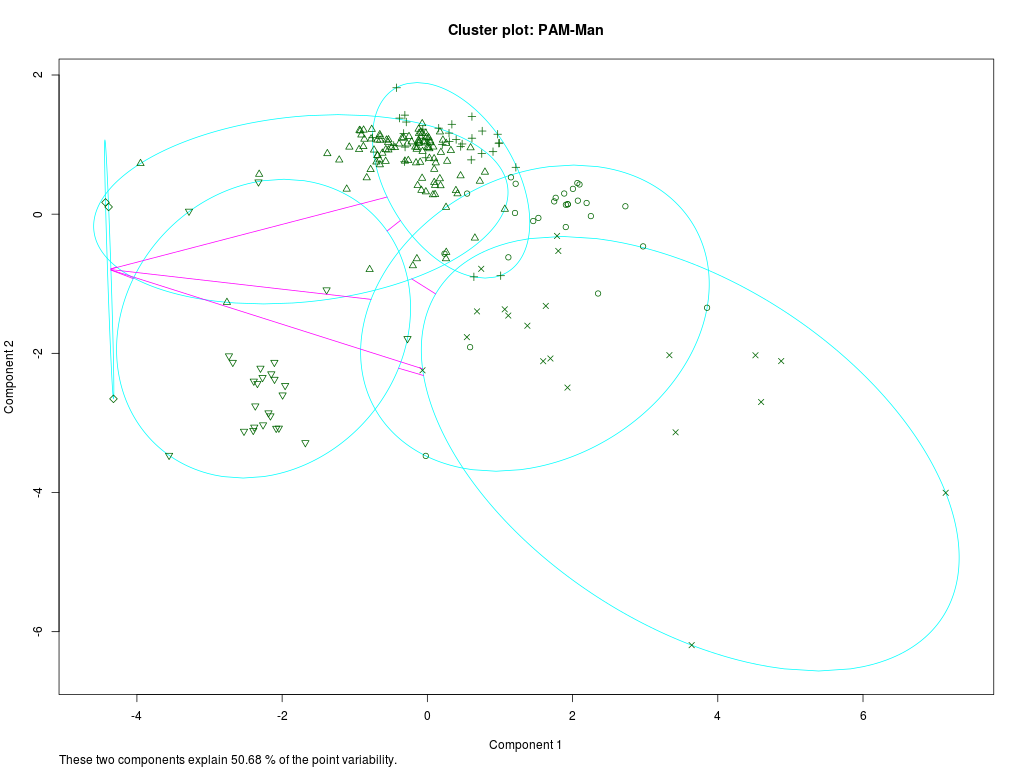
\includegraphics[width=0.8\textwidth]{resources/plots/glass_PAM-Man_cluster.png}
      \caption{Klastry dla algorytmu PAM (Manhattan) dla zbioru "Glass".}
    \end{figure}

\subsection{Zbiór "Wine"}
  \begin{figure}[H]
    \center
    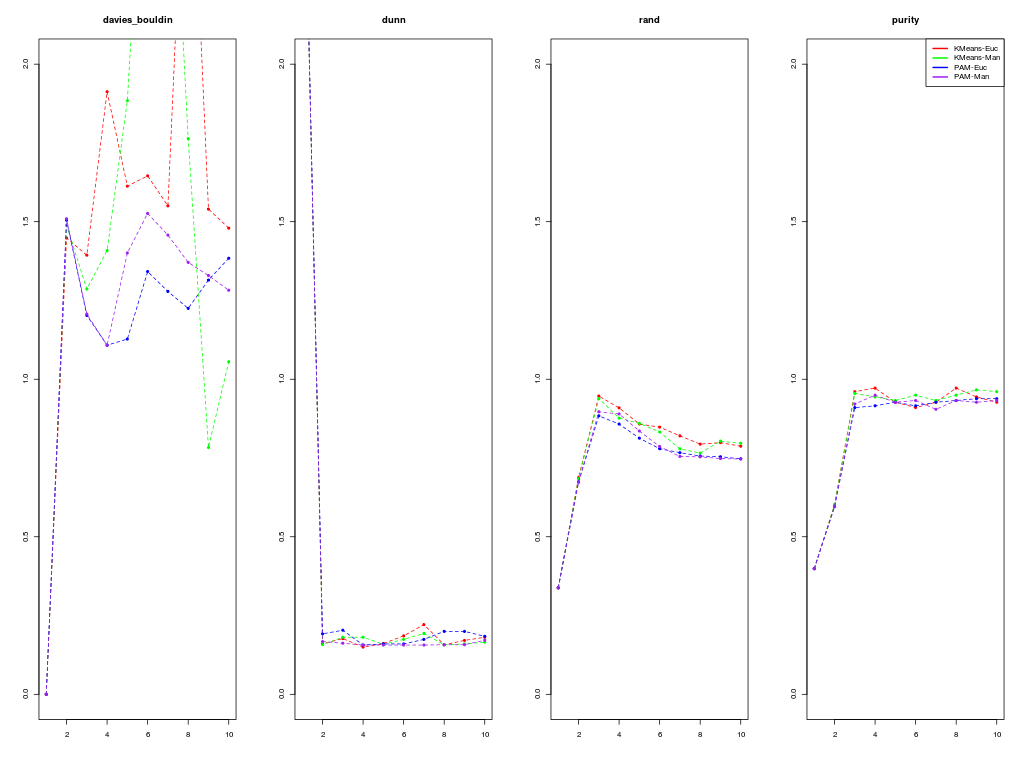
\includegraphics[width=\textwidth]{resources/plots/wine_metrics.png}
    \caption{Wykresy wartości metryk dla zbioru "Wine".}
  \end{figure}

  % latex table generated in R 3.4.4 by xtable 1.8-2 package
% Sun May  6 16:30:42 2018
\begin{table}[ht]
\centering
\begin{tabular}{llrlrr}
  \hline
alg & nb\_clus & davies\_bouldin & dunn & rand & purity \\ 
  \hline
KMeans-Euc & 1 & 0.00 & INF & 0.34 & 0.40 \\ 
  KMeans-Euc & 2 & 1.45 & 0.16 & 0.69 & 0.60 \\ 
  KMeans-Euc & 3 & 1.39 & 0.177 & 0.95 & 0.96 \\ 
  KMeans-Euc & 4 & 1.91 & 0.15 & 0.91 & 0.97 \\ 
  KMeans-Euc & 5 & 1.61 & 0.161 & 0.86 & 0.93 \\ 
  KMeans-Euc & 6 & 1.65 & 0.185 & 0.85 & 0.91 \\ 
  KMeans-Euc & 7 & 1.55 & 0.221 & 0.82 & 0.93 \\ 
  KMeans-Euc & 8 & 2.08 & 0.157 & 0.79 & 0.97 \\ 
  KMeans-Euc & 9 & 1.54 & 0.171 & 0.80 & 0.94 \\ 
  KMeans-Euc & 10 & 1.48 & 0.181 & 0.79 & 0.93 \\ 
  KMeans-Man & 1 & 0.00 & INF & 0.34 & 0.40 \\ 
  KMeans-Man & 2 & 1.49 & 0.158 & 0.69 & 0.60 \\ 
  KMeans-Man & 3 & 1.29 & 0.181 & 0.94 & 0.95 \\ 
  KMeans-Man & 4 & 1.41 & 0.181 & 0.88 & 0.94 \\ 
  KMeans-Man & 5 & 1.88 & 0.158 & 0.86 & 0.93 \\ 
  KMeans-Man & 6 & 2.06 & 0.174 & 0.83 & 0.95 \\ 
  KMeans-Man & 7 & 2.07 & 0.193 & 0.78 & 0.93 \\ 
  KMeans-Man & 8 & 1.76 & 0.157 & 0.77 & 0.95 \\ 
  KMeans-Man & 9 & 0.78 & 0.16 & 0.80 & 0.97 \\ 
  KMeans-Man & 10 & 1.06 & 0.165 & 0.80 & 0.96 \\ 
  PAM-Euc & 1 & 0.00 & INF & 0.34 & 0.40 \\ 
  PAM-Euc & 2 & 1.50 & 0.192 & 0.67 & 0.60 \\ 
  PAM-Euc & 3 & 1.20 & 0.203 & 0.88 & 0.91 \\ 
  PAM-Euc & 4 & 1.11 & 0.156 & 0.86 & 0.92 \\ 
  PAM-Euc & 5 & 1.13 & 0.16 & 0.81 & 0.93 \\ 
  PAM-Euc & 6 & 1.34 & 0.16 & 0.78 & 0.92 \\ 
  PAM-Euc & 7 & 1.28 & 0.174 & 0.77 & 0.93 \\ 
  PAM-Euc & 8 & 1.23 & 0.2 & 0.76 & 0.93 \\ 
  PAM-Euc & 9 & 1.31 & 0.2 & 0.75 & 0.94 \\ 
  PAM-Euc & 10 & 1.38 & 0.184 & 0.75 & 0.94 \\ 
  PAM-Man & 1 & 0.00 & INF & 0.34 & 0.40 \\ 
  PAM-Man & 2 & 1.51 & 0.167 & 0.67 & 0.60 \\ 
  PAM-Man & 3 & 1.21 & 0.162 & 0.90 & 0.92 \\ 
  PAM-Man & 4 & 1.11 & 0.156 & 0.89 & 0.95 \\ 
  PAM-Man & 5 & 1.40 & 0.156 & 0.84 & 0.93 \\ 
  PAM-Man & 6 & 1.53 & 0.156 & 0.79 & 0.93 \\ 
  PAM-Man & 7 & 1.46 & 0.156 & 0.76 & 0.90 \\ 
  PAM-Man & 8 & 1.37 & 0.157 & 0.75 & 0.93 \\ 
  PAM-Man & 9 & 1.33 & 0.157 & 0.75 & 0.93 \\ 
  PAM-Man & 10 & 1.28 & 0.172 & 0.75 & 0.93 \\ 
   \hline
\end{tabular}
\end{table}


  \subsubsection{Algorytm K-Means (Euclidean)} 
    \begin{figure}[H]
      \center
      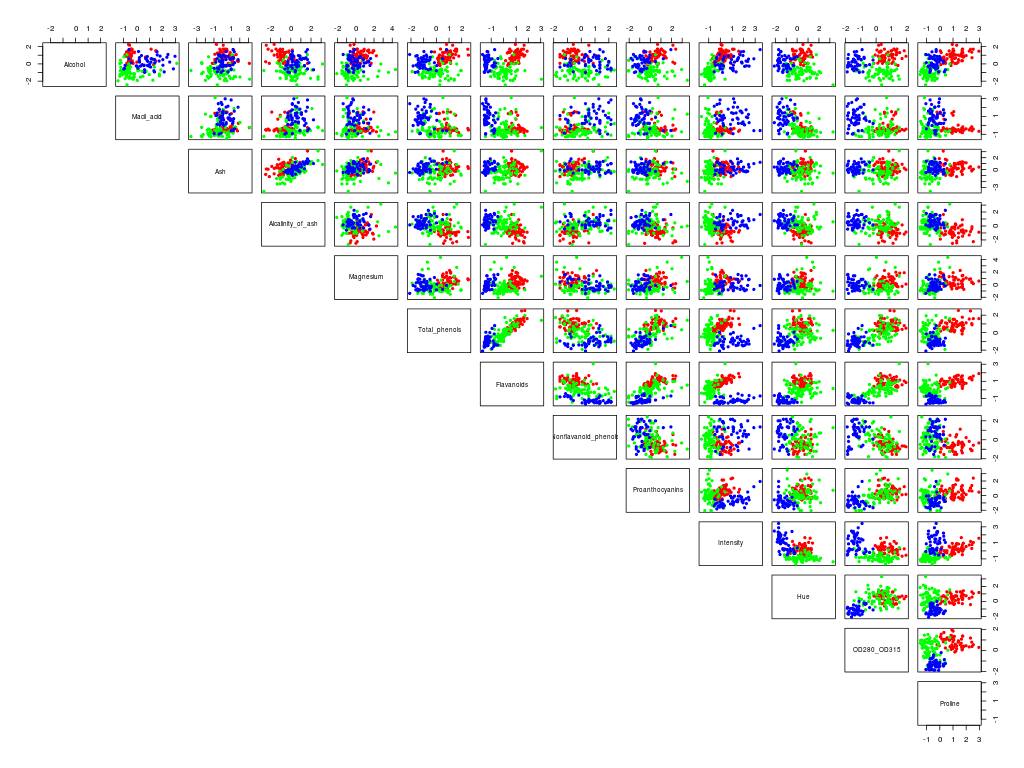
\includegraphics[width=0.8\textwidth]{resources/plots/wine_KMeans-Euc_scatter.png}
      \caption{Wynik klasteryzacji dla algorytmu KMeans (Euclidean) dla zbioru "Wine".}
    \end{figure}
    \begin{figure}[H]
      \center
      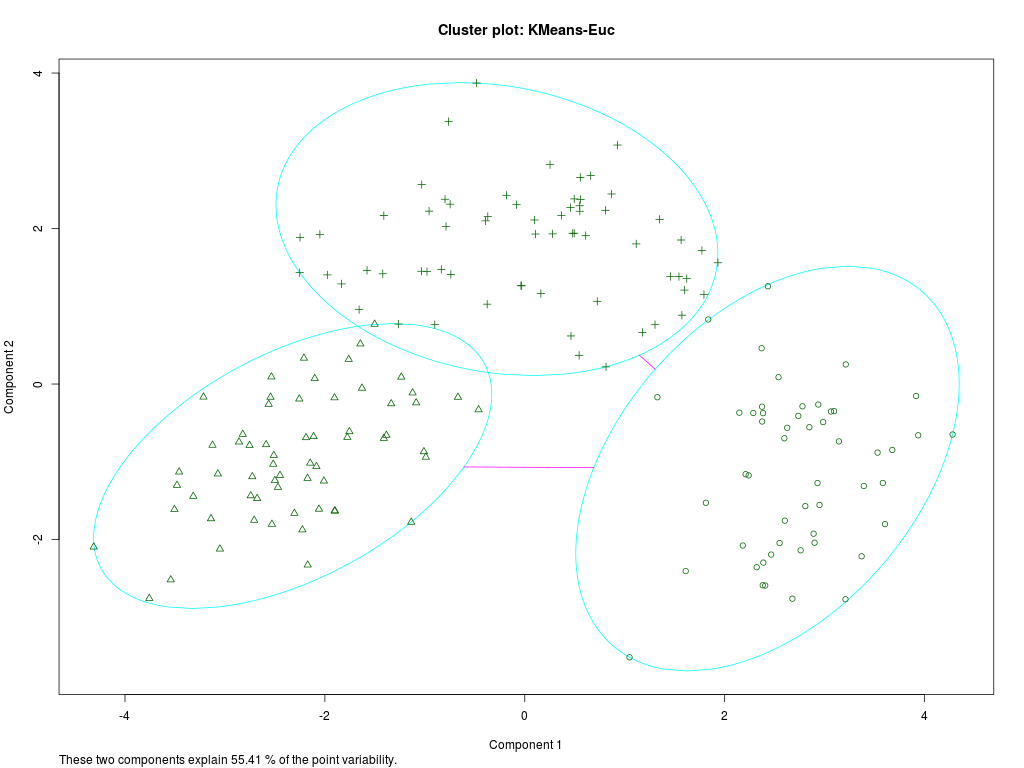
\includegraphics[width=0.8\textwidth]{resources/plots/wine_KMeans-Euc_cluster.png}
      \caption{Klastry dla algorytmu KMeans (Euclidean) dla zbioru "Wine".}
    \end{figure}

  \subsubsection{Algorytm K-Means (Manhattan)} 
    \begin{figure}[H]
      \center
      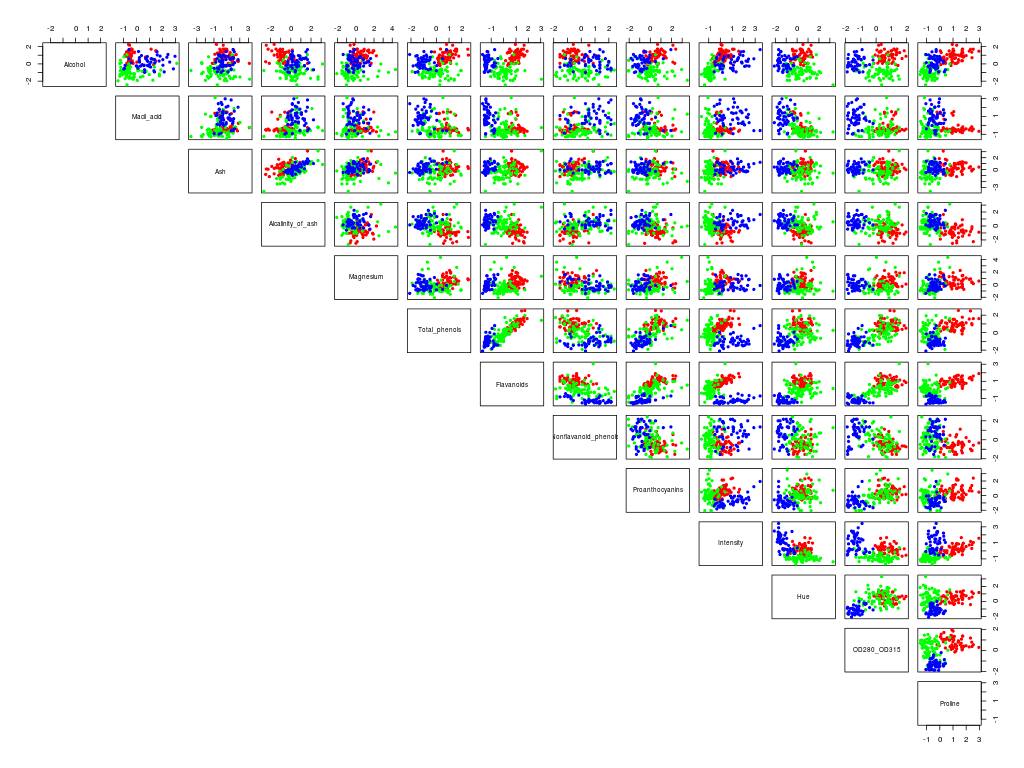
\includegraphics[width=0.8\textwidth]{resources/plots/wine_KMeans-Man_scatter.png}
      \caption{Wynik klasteryzacji dla algorytmu KMeans (Manhattan) dla zbioru "Wine".}
    \end{figure}
    \begin{figure}[H]
      \center
      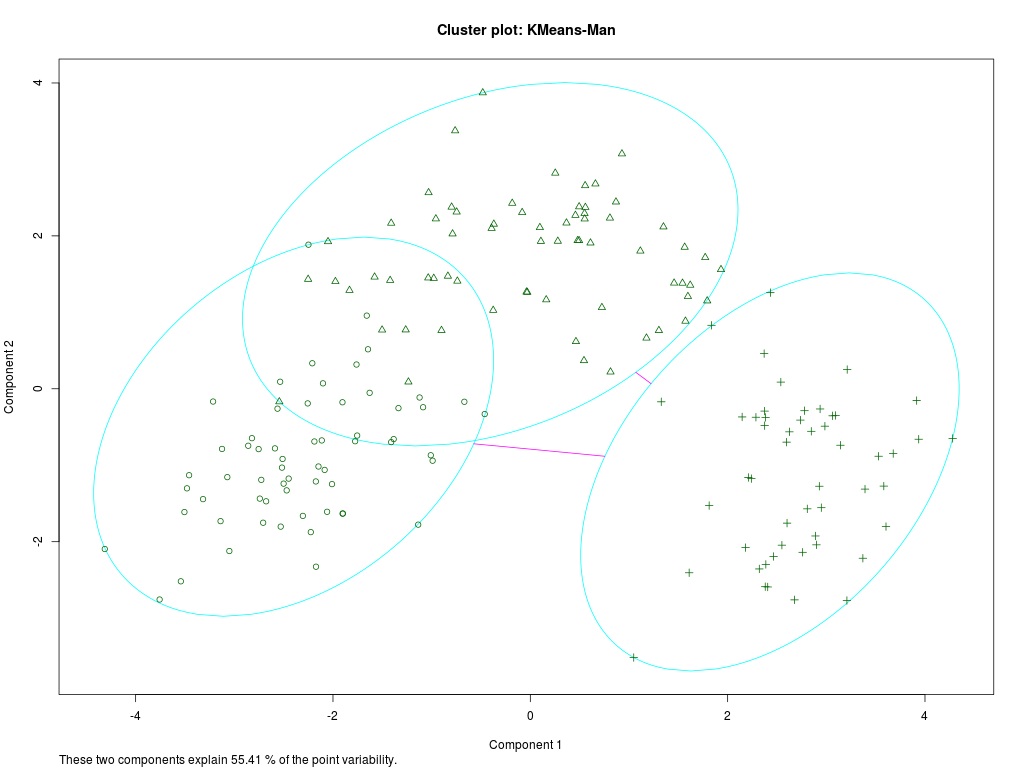
\includegraphics[width=0.8\textwidth]{resources/plots/wine_KMeans-Man_cluster.png}
      \caption{Klastry dla algorytmu KMeans (Manhattan) dla zbioru "Wine".}
    \end{figure}

  \subsubsection{Algorytm PAM (Euclidean)} 
    \begin{figure}[H]
      \center
      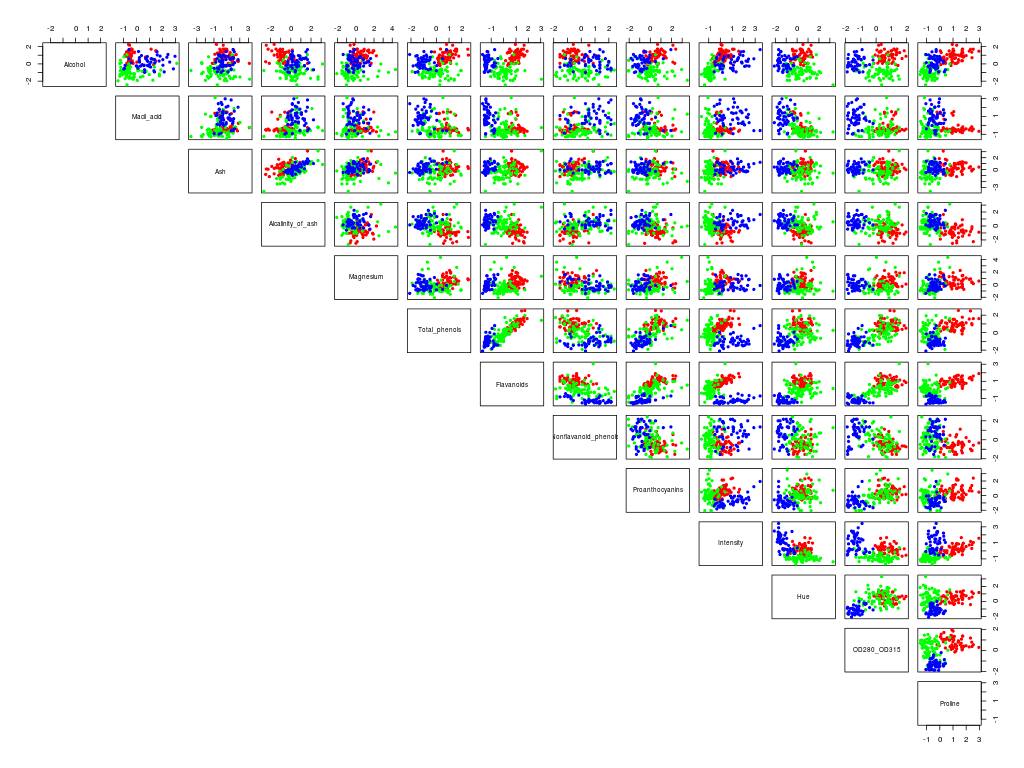
\includegraphics[width=0.8\textwidth]{resources/plots/wine_PAM-Euc_scatter.png}
      \caption{Wynik klasteryzacji dla algorytmu PAM (Euclidean) dla zbioru "Wine".}
    \end{figure}
    \begin{figure}[H]
      \center
      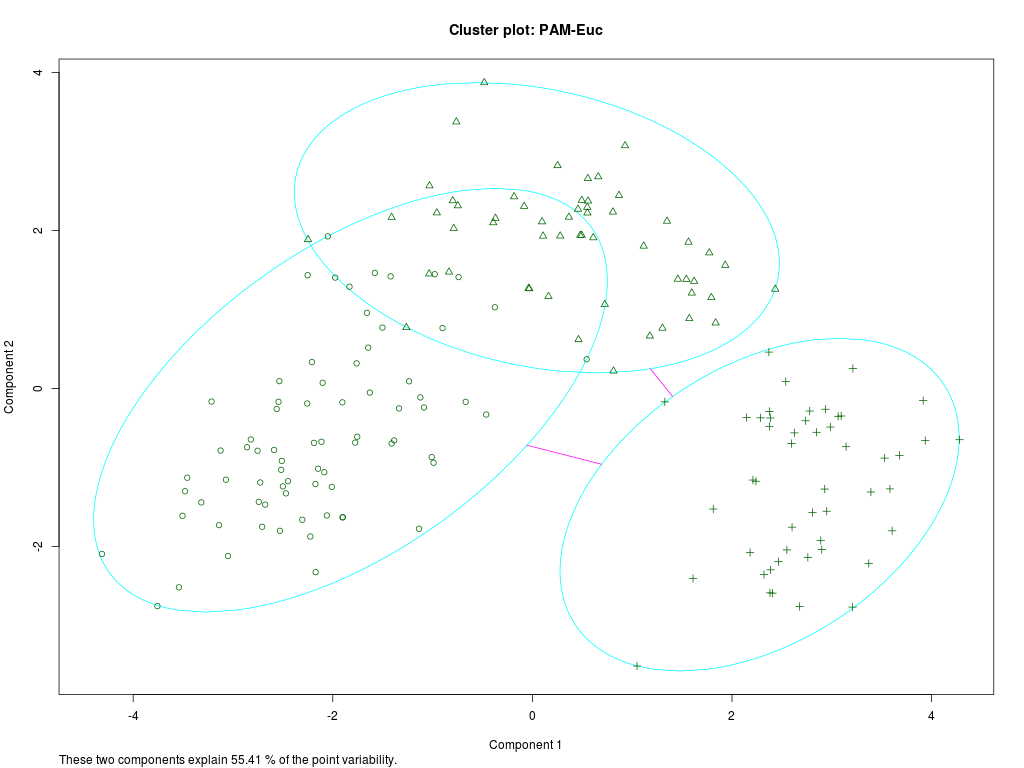
\includegraphics[width=0.8\textwidth]{resources/plots/wine_PAM-Euc_cluster.png}
      \caption{Klastry dla algorytmu PAM (Euclidean) dla zbioru "Wine".}
    \end{figure}

  \subsubsection{Algorytm PAM (Manhattan)} 
    \begin{figure}[H]
      \center
      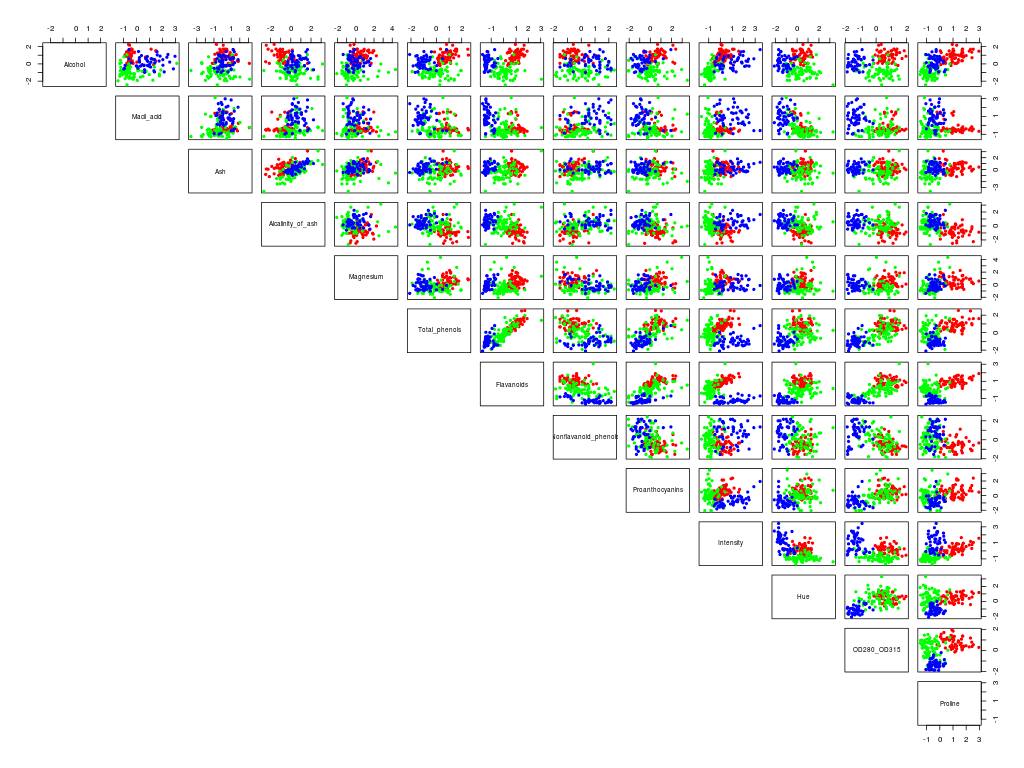
\includegraphics[width=0.8\textwidth]{resources/plots/wine_PAM-Man_scatter.png}
      \caption{Wynik klasteryzacji dla algorytmu PAM (Manhattan) dla zbioru "Wine".}
    \end{figure}
    \begin{figure}[H]
      \center
      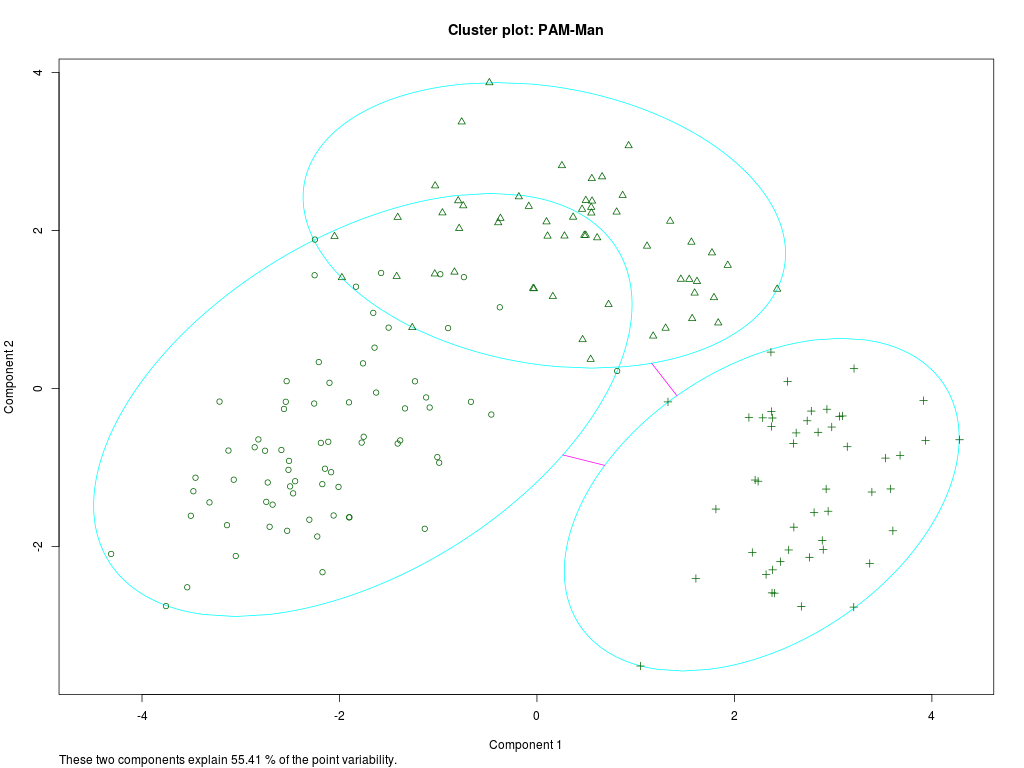
\includegraphics[width=0.8\textwidth]{resources/plots/wine_PAM-Man_cluster.png}
      \caption{Klastry dla algorytmu PAM (Manhattan) dla zbioru "Wine".}
    \end{figure}

\subsection{Zbiór "Seeds"}
  \begin{figure}[H]
    \center
    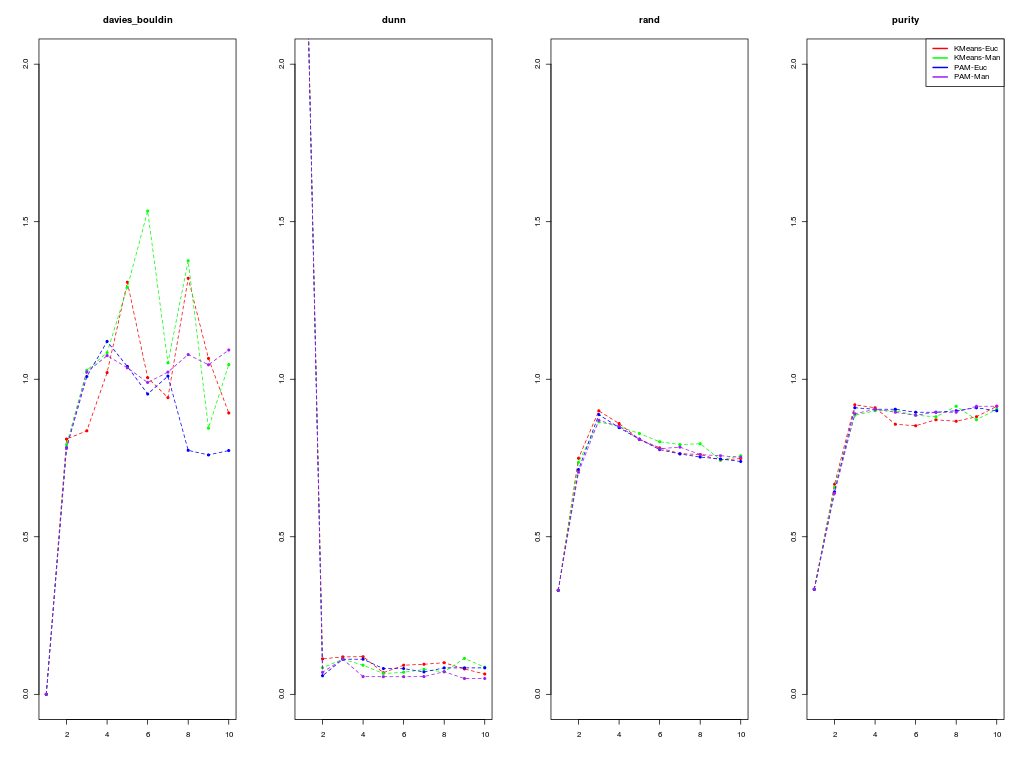
\includegraphics[width=\textwidth]{resources/plots/seeds_metrics.png}
    \caption{Wykresy wartości metryk dla zbioru "Seeds".}
  \end{figure}

  % latex table generated in R 3.4.4 by xtable 1.8-2 package
% Sun May  6 16:31:33 2018
\begin{table}[ht]
\centering
\begin{tabular}{llrlrr}
  \hline
alg & nb\_clus & davies\_bouldin & dunn & rand & purity \\ 
  \hline
KMeans-Euc & 1 & 0.00 & INF & 0.33 & 0.33 \\ 
  KMeans-Euc & 2 & 0.81 & 0.113 & 0.75 & 0.67 \\ 
  KMeans-Euc & 3 & 0.84 & 0.119 & 0.90 & 0.92 \\ 
  KMeans-Euc & 4 & 1.02 & 0.119 & 0.86 & 0.91 \\ 
  KMeans-Euc & 5 & 1.31 & 0.069 & 0.81 & 0.86 \\ 
  KMeans-Euc & 6 & 1.00 & 0.092 & 0.78 & 0.85 \\ 
  KMeans-Euc & 7 & 0.94 & 0.095 & 0.76 & 0.87 \\ 
  KMeans-Euc & 8 & 1.32 & 0.1 & 0.76 & 0.87 \\ 
  KMeans-Euc & 9 & 1.07 & 0.081 & 0.74 & 0.88 \\ 
  KMeans-Euc & 10 & 0.89 & 0.064 & 0.75 & 0.91 \\ 
  KMeans-Man & 1 & 0.00 & INF & 0.33 & 0.33 \\ 
  KMeans-Man & 2 & 0.79 & 0.084 & 0.74 & 0.66 \\ 
  KMeans-Man & 3 & 1.03 & 0.111 & 0.86 & 0.89 \\ 
  KMeans-Man & 4 & 1.08 & 0.092 & 0.85 & 0.90 \\ 
  KMeans-Man & 5 & 1.29 & 0.066 & 0.83 & 0.90 \\ 
  KMeans-Man & 6 & 1.53 & 0.07 & 0.80 & 0.89 \\ 
  KMeans-Man & 7 & 1.05 & 0.079 & 0.79 & 0.88 \\ 
  KMeans-Man & 8 & 1.38 & 0.071 & 0.80 & 0.91 \\ 
  KMeans-Man & 9 & 0.84 & 0.114 & 0.74 & 0.87 \\ 
  KMeans-Man & 10 & 1.05 & 0.086 & 0.76 & 0.91 \\ 
  PAM-Euc & 1 & 0.00 & INF & 0.33 & 0.33 \\ 
  PAM-Euc & 2 & 0.78 & 0.059 & 0.71 & 0.64 \\ 
  PAM-Euc & 3 & 1.01 & 0.111 & 0.89 & 0.91 \\ 
  PAM-Euc & 4 & 1.12 & 0.111 & 0.85 & 0.91 \\ 
  PAM-Euc & 5 & 1.04 & 0.082 & 0.81 & 0.91 \\ 
  PAM-Euc & 6 & 0.95 & 0.082 & 0.78 & 0.90 \\ 
  PAM-Euc & 7 & 1.01 & 0.071 & 0.76 & 0.90 \\ 
  PAM-Euc & 8 & 0.77 & 0.084 & 0.75 & 0.90 \\ 
  PAM-Euc & 9 & 0.76 & 0.084 & 0.75 & 0.91 \\ 
  PAM-Euc & 10 & 0.77 & 0.084 & 0.74 & 0.90 \\ 
  PAM-Man & 1 & 0.00 & INF & 0.33 & 0.33 \\ 
  PAM-Man & 2 & 0.78 & 0.07 & 0.70 & 0.64 \\ 
  PAM-Man & 3 & 1.02 & 0.111 & 0.87 & 0.89 \\ 
  PAM-Man & 4 & 1.07 & 0.056 & 0.85 & 0.91 \\ 
  PAM-Man & 5 & 1.04 & 0.056 & 0.81 & 0.90 \\ 
  PAM-Man & 6 & 0.99 & 0.056 & 0.78 & 0.89 \\ 
  PAM-Man & 7 & 1.02 & 0.056 & 0.79 & 0.90 \\ 
  PAM-Man & 8 & 1.08 & 0.072 & 0.76 & 0.90 \\ 
  PAM-Man & 9 & 1.05 & 0.05 & 0.76 & 0.91 \\ 
  PAM-Man & 10 & 1.09 & 0.05 & 0.75 & 0.91 \\ 
   \hline
\end{tabular}
\end{table}


  \subsubsection{Algorytm K-Means (Euclidean)} 
    \begin{figure}[H]
      \center
      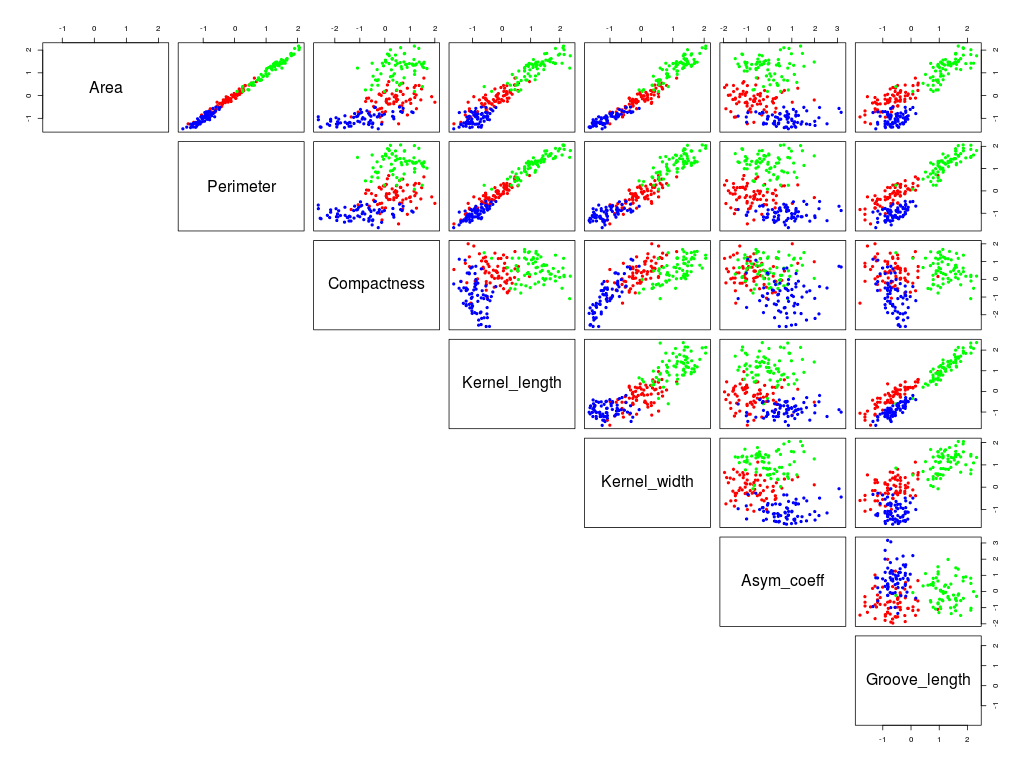
\includegraphics[width=0.8\textwidth]{resources/plots/seeds_KMeans-Euc_scatter.png}
      \caption{Wynik klasteryzacji dla algorytmu KMeans (Euclidean) dla zbioru "Seeds".}
    \end{figure}
    \begin{figure}[H]
      \center
      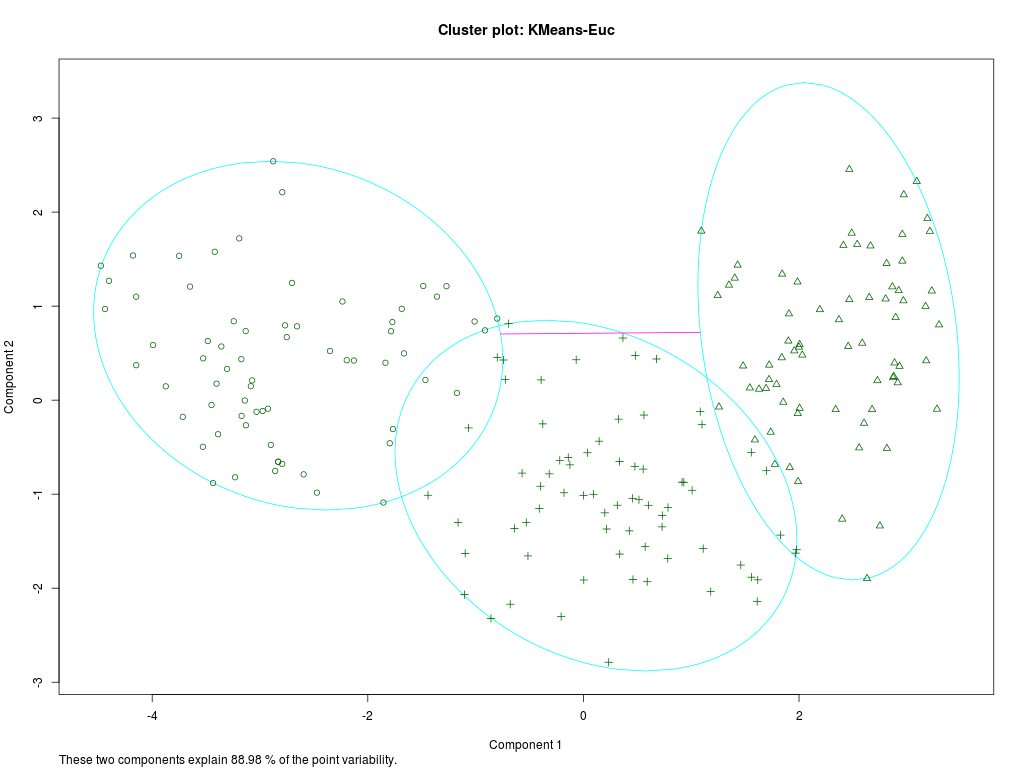
\includegraphics[width=0.8\textwidth]{resources/plots/seeds_KMeans-Euc_cluster.png}
      \caption{Klastry dla algorytmu KMeans (Euclidean) dla zbioru "Seeds".}
    \end{figure}

  \subsubsection{Algorytm K-Means (Manhattan)} 
    \begin{figure}[H]
      \center
      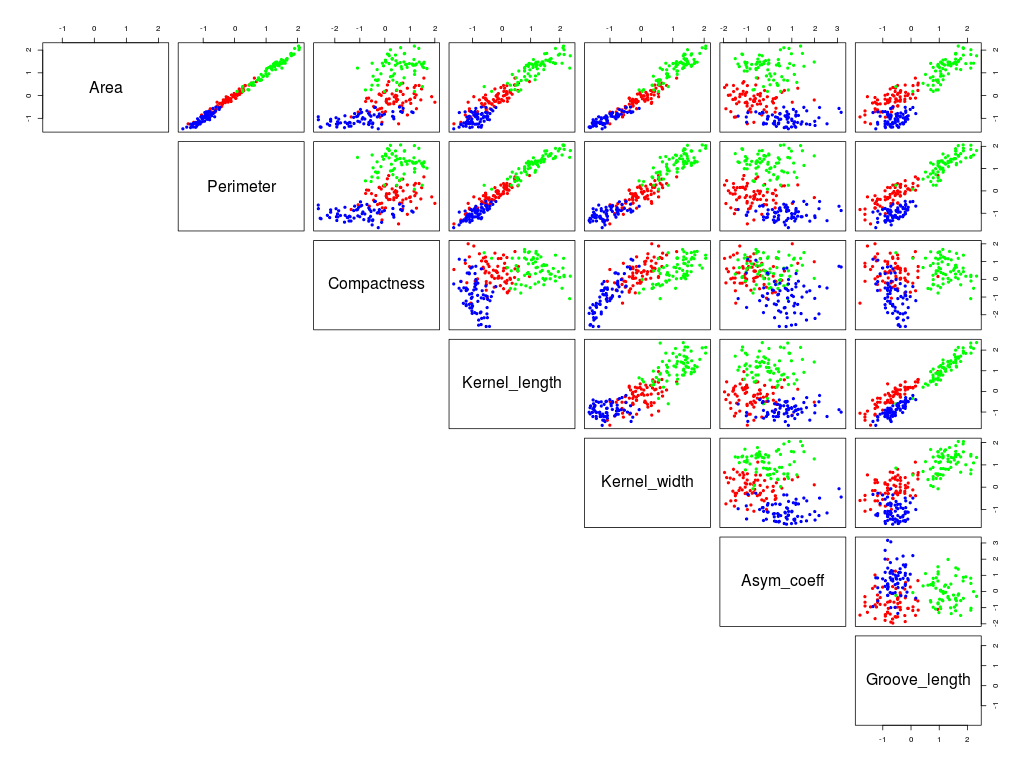
\includegraphics[width=0.8\textwidth]{resources/plots/seeds_KMeans-Man_scatter.png}
      \caption{Wynik klasteryzacji dla algorytmu KMeans (Manhattan) dla zbioru "Seeds".}
    \end{figure}
    \begin{figure}[H]
      \center
      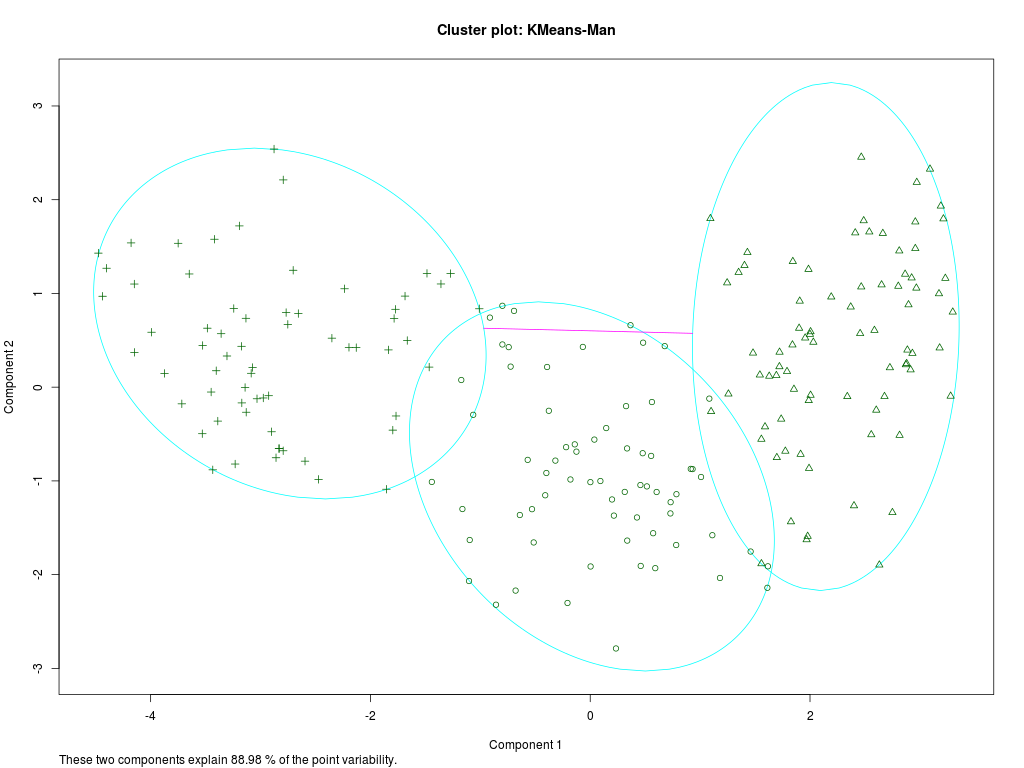
\includegraphics[width=0.8\textwidth]{resources/plots/seeds_KMeans-Man_cluster.png}
      \caption{Klastry dla algorytmu KMeans (Manhattan) dla zbioru "Seeds".}
    \end{figure}

  \subsubsection{Algorytm PAM (Euclidean)} 
    \begin{figure}[H]
      \center
      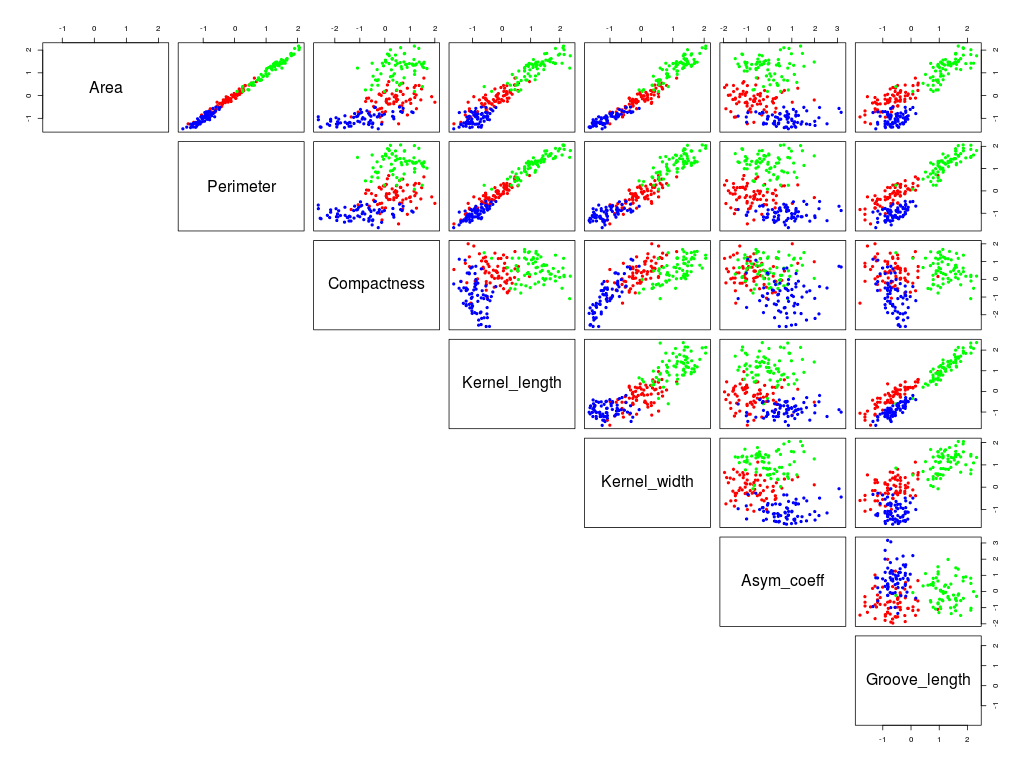
\includegraphics[width=0.8\textwidth]{resources/plots/seeds_PAM-Euc_scatter.png}
      \caption{Wynik klasteryzacji dla algorytmu PAM (Euclidean) dla zbioru "Seeds".}
    \end{figure}
    \begin{figure}[H]
      \center
      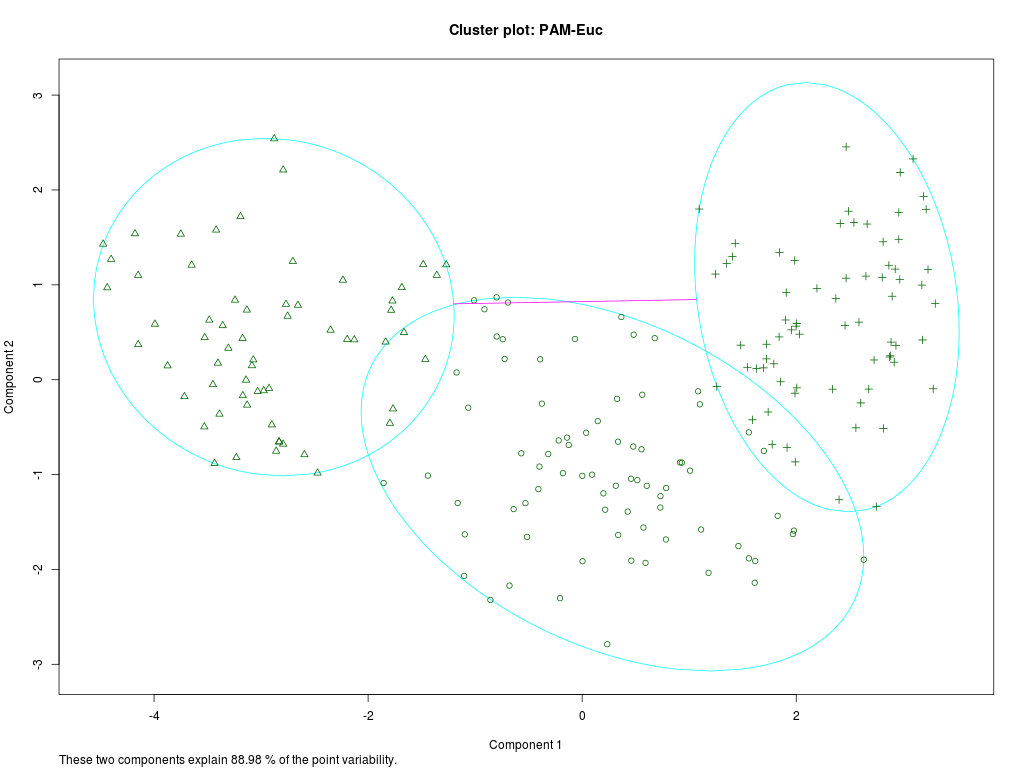
\includegraphics[width=0.8\textwidth]{resources/plots/seeds_PAM-Euc_cluster.png}
      \caption{Klastry dla algorytmu PAM (Euclidean) dla zbioru "Seeds".}
    \end{figure}

  \subsubsection{Algorytm PAM (Manhattan)} 
    \begin{figure}[H]
      \center
      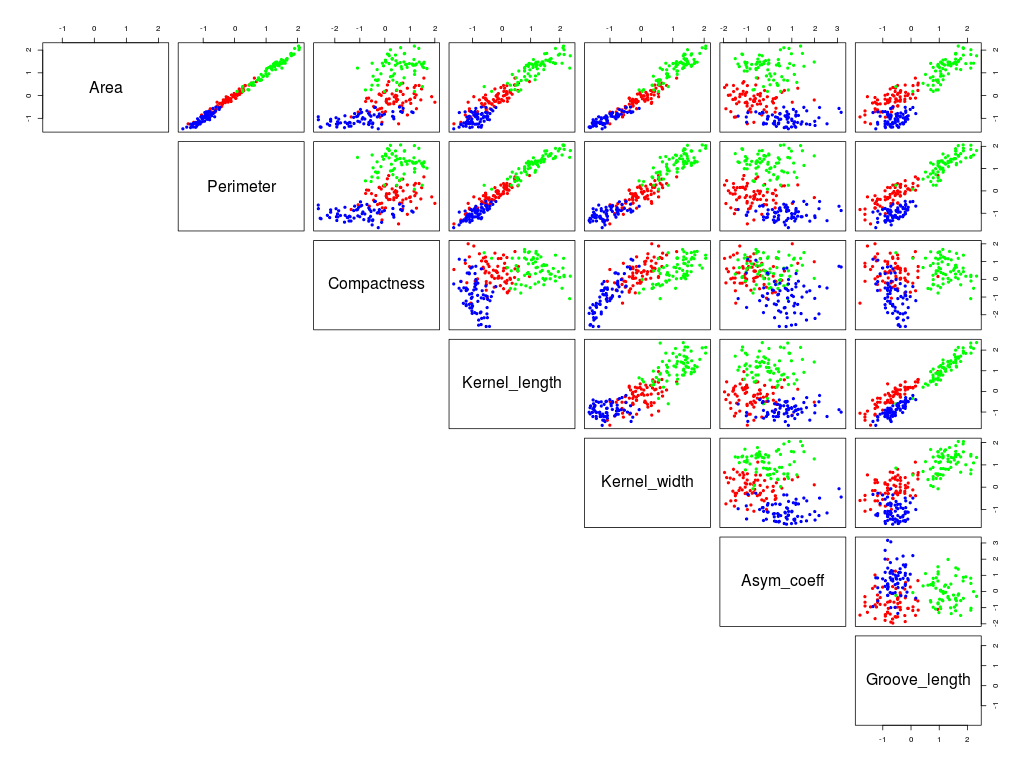
\includegraphics[width=0.8\textwidth]{resources/plots/seeds_PAM-Man_scatter.png}
      \caption{Wynik klasteryzacji dla algorytmu PAM (Manhattan) dla zbioru "Seeds".}
    \end{figure}
    \begin{figure}[H]
      \center
      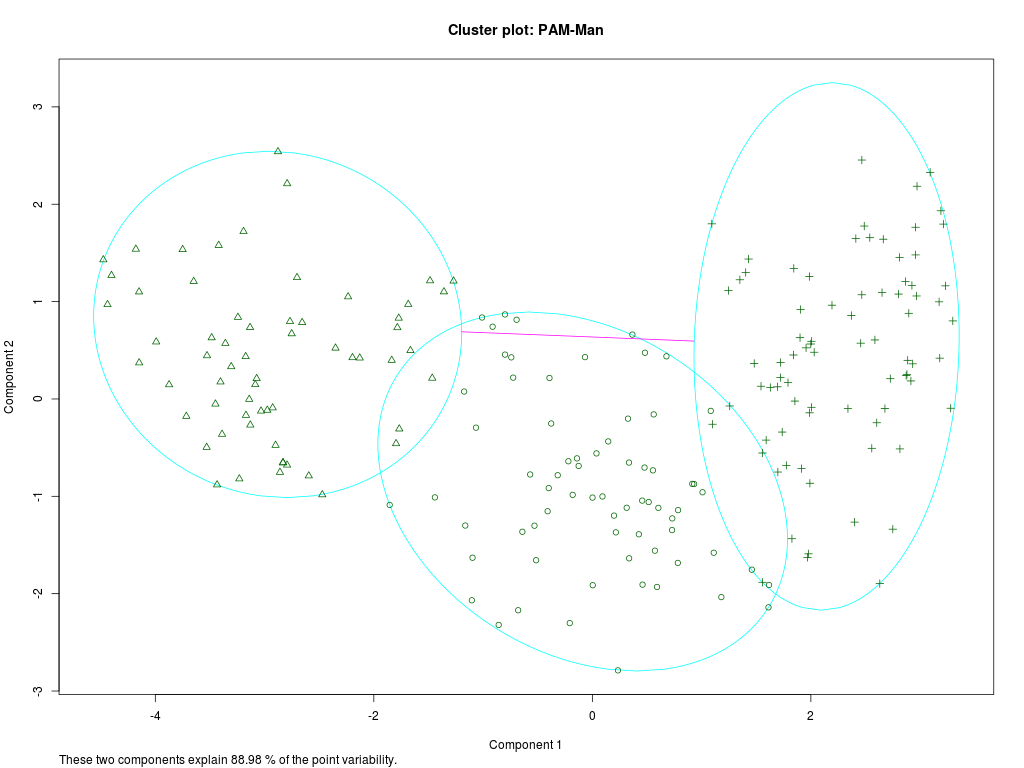
\includegraphics[width=0.8\textwidth]{resources/plots/seeds_PAM-Man_cluster.png}
      \caption{Klastry dla algorytmu PAM (Manhattan) dla zbioru "Seeds".}
    \end{figure}


\subsection{Kroswalidacja Seeds}
Przeprowadzono kroswalidację dla zbioru \textit{Seeds} z użyciem algorytmu Kmeans z parametrami: liczba grup = 3 (liczba klas), metryka euklidesowa.
Zbadano wartości miar \textit{Balanced Accuracy}, \textit{Precision}, \textit{Recall} oraz \textit{F1} dla kroswalidacji kolejno 2, 3, ..., 10-fold.
Wyniki pomiarów zostały przedstawione poniżej:

\begin{figure}[H]
  \center
  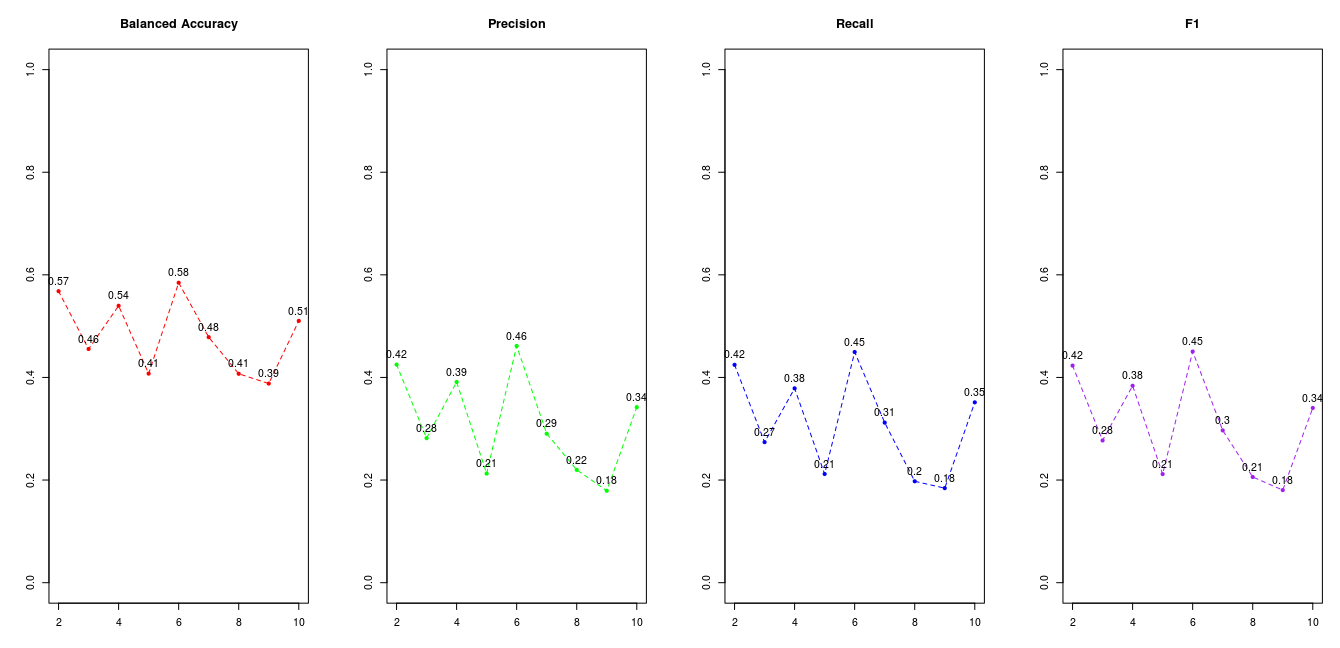
\includegraphics[width=\textwidth]{resources/cv.png}
  \caption{Wyniki kroswalidacji dla zbioru \textit{Seeds}.}
\end{figure}
